\documentclass[7pt,landscape, margin = 0.1mm]{article}
\usepackage{amssymb,amsmath,amsthm,amsfonts}
\usepackage{multicol,multirow}
\usepackage{graphicx}
\usepackage[dvipsnames]{xcolor}
% Tables
\usepackage{tabularx, multirow}
\usepackage{booktabs}
\renewcommand*{\arraystretch}{2}
\usepackage{float}
\usepackage{calc}
\usepackage{soul}
\usepackage[dvipsnames]{xcolor}
\usepackage{ifthen}
\usepackage{titlesec}
\usepackage[landscape]{geometry}
\usepackage{enumitem}
\usepackage{syntonly}
\setitemize{noitemsep,topsep=0pt,parsep=0pt,partopsep=0pt}
\usepackage[colorlinks=true,citecolor=blue,linkcolor=blue]{hyperref}
\usepackage{tikz}
\def\cm{\tikz\fill[scale=0.4](0,.35) -- (.25,0) -- (1,.7) -- (.25,.15) -- cycle;} 
\ifthenelse{\lengthtest { \paperwidth = 11in}}
    { \geometry{top=.1in,left=.1in,right=.1in,bottom=.1in} }
	{\ifthenelse{ \lengthtest{ \paperwidth = 297mm}}
		{\geometry{top=1mm,left=1mm,right=1mm,bottom=1mm} }
		{\geometry{top=1mm,left=1mm,right=1mm,bottom=1mm} }
	}

\pagestyle{empty}
\def\limn{\lim_{n\to \infty}}
\def\limxo{\lim_{x\to 0}}
\def\limxi{\lim_{x\to\infty}}
\def\limxn{\lim_{x\to-\infty}}
\def\sumk{\sum_{k=1}^\infty}
\def\sumn{\sum_{n=0}^\infty}
\def\R{\mathbb{R}}
\def\dx{\text{ d}x}
%\definecolor{col1}{rgb}{0.00, 0.03,0.45}
%\definecolor{col2}{rgb}{0.27, 0.00, 0.31}
%\definecolor{col3}{rgb}{0.32, 0.00, 0.19}
%\definecolor{col4}{rgb}{0.30, 0.00, 0.09}
%\definecolor{col5}{rgb}{0.27, 0.00, 0.01}

\makeatletter

 

\newcommand{\nextcol}{\vfill\null\columnbreak}

\newcommand{\titellinie}{\rule{1.\linewidth}{0.75pt}}

\titleformat{\subsection}
  {\normalfont\fontsize{10}{10}\bfseries}{\thesection}{1em}{}

\newcommand*{\mysection}[2][black]{\vskip 0pt \titellinie\vspace{-20pt}\section{#2}\vspace{-14pt}\titellinie \colorlet{chaptecolor}{#1}}

\newcommand*{\mysubsection}[1]{\vspace{-2mm}\color{chaptercolor}\subsection{ #1 }
\vspace{-1mm}\hrule\vspace{1.5mm}\color{black}
\vspace{2mm}}

\newcommand{\COL}[1]{ \color{chaptercolor} \bf{#1}\color{black}     \\}


\newcommand{\KRZ}[2]{\vspace{1mm} \hline \vspace{1mm} \color{chaptercolor}{RC #1}:\color{black} \   \hspace{0.2cm}\vspace{1mm}   {\begin{minipage}{20em}
#2 \end{minipage}} \vspace{1mm}  \hline \vspace{1mm}  \\}


\newcommand{\DEF}[2]{\color{chaptercolor}\bf{Def #1}:\color{black}    \hspace{0.2cm} #2 \\}

\newcommand{\NOTE}[2]{\color{chaptercolor}\bf{Note #1}:\color{black}    \hspace{0.2cm} #2 \\}

\newcommand{\COR}[2]{\color{chaptercolor}\bf{Cor #1}:\color{black}    \hspace{0.2cm} #2 \\}

\newcommand{\LEM}[2]{\color{chaptercolor}\bf{Lem #1}:\color{black}    \hspace{0.2cm} #2 \\}

\newcommand{\THE}[2]{\color{chaptercolor}\bf{Trm #1}:\color{black}    \hspace{0.2cm} #2 \\}
\newcommand{\SA}[2]{\color{chaptercolor}\bf{S #1}:\color{black}    \hspace{0.2cm} #2 \\}
\newcommand{\AX}[2]{\color{chaptercolor}\bf{Axm #1}:\color{black}    \hspace{0.2cm} #2 \\}

\makeatother
\setcounter{secnumdepth}{0}
\setlength{\parindent}{0pt}
\setlength{\parskip}{0pt plus 0.5ex}
\setlength{\marginparwidth}{0pt}
\setlength{\marginparsep}{0pt}
% -----------------------------------------------------------------------
\begin{document}
\syntaxonly
\centering
\pagenumbering{arabic}
\raggedcolumns

\scriptsize

\begin{center}
     \Large{\textbf{Cheat Sheet}: Comp Sc BSc, Analysis} \\
\end{center}
\begin{multicols}{4}
\setlength{\premulticols}{0.5pt}
\setlength{\postmulticols}{0.5pt}
\setlength{\multicolsep}{0.5pt}
\setlength{\columnsep}{0.2pt}
\setlength{\columnseprule}{0.4pt}

\begin{flushleft}

\mysection[red]{\centering Zahlenräume}
\mysubsection{Reelle Zahlen}
\DEF{(Reelle Zahlen)}{Es gibt eine Menge $\mathbb{R}$ mit:
\begin{itemize}
\item $+: \mathbb{R} \mapsto \mathbb{R}$ (Addition)
\item $\cdot : \mathbb{R} \mapsto \mathbb{R}$ (Multiplikation)
\item $\leq$ (Ordnungsrelation)}
\end{itemize}
\SA{1.1.2}{$\mathbb{R}$ ist ein kommutativer, angeordneter Körper, der ordnungsvollständig ist.}
\AX{$\mathbb{R}$}{Folgende Axiome gelten für $\mathbb{R}$ und $\mathbb{Q}$:
\begin{itemize}
\item \COL{Axiome der Addition $(A)$}
\begin{itemize}
\item[$(A1)$] Assoziativität: $x + (y + z) = (x+y)+z \; \; \; \forall x,y,z, \in \mathbb{R}$
\item[$(A2)$] Neutrales Element:$x + 0 = x \; \; \; \forall x \in \mathbb{R}$
\item [$(A3)$] Inverses Element:$\forall x \in \mathbb{R} \; \exists y \in \mathbb{R}: x+y = 0$
\item Inverses ist eindeutig und man schreibt: $-x$
\item[$(A4)$] Kommutativität:$x+z = z+x \; \; \; \forall x,z \in \mathbb{R}$
\end{itemize}
\item \COL{Axiome der Multiplikation $(M)$}
\begin{itemize}
\item[$(M1)$] Assoziativität:$x \cdot (y \cdot z) = (x\cdot y)\cdot z \; \; \; \forall x,y,z, \in \mathbb{R}$
\item[$(M2)$]: Neutrales Element:$x \cdot 1 = x \; \; \; \forall x \in \mathbb{R}$
\item[$(M3)$] Inverses Element:$\forall x \in \mathbb{R} , x \neq 0\; \exists y \in \mathbb{R}: x \cdot y = 1$
\item Inverse ist eindeutig und man schreibt: $x^{-1}$
\item[$(M4)$] Kommutativität:$x \cdot z = z \cdot x \; \; \; \forall x,z \in \mathbb{R}$
\end{itemize}
\item \COL{Ordnungsaxiome $(O)$}
\begin{itemize}
\item[$(O1)$] Reflexivität:$x \leq x \; \; \; \forall x \in \mathbb{R}$
\item[$(O2)$] Transitivität:$x \leq y$ und $y \leq z \Rightarrow x \leq z$
\item[$(O3)$] Antisymmetrie:$x \leq y$ und $y \leq x \Rightarrow x = y$
\item[$(O4)$] Total:$\forall x,y \in \mathbb{R}$ gilt entweder $x \leq y$ oder $x \geq y$
\end{itemize}
\item \COL{Distributivität $(D)$}
\begin{itemize}
\item[$(D1)$] Distributivität:$x \cdot (y + z) = x \cdot y + x \cdot z \; \; \; \forall x,y,z \in \mathbb{R}$
\end{itemize}
\item \COL{Kompabilität $(K)$}
\begin{itemize}
\item[$(K1)$] $\forall x,y,z \in \mathbb{R}: x \leq y \Rightarrow x + z \leq y + z$:$(K2)$: $\forall x \geq 0 , \forall y \geq 0: x \cdot y \geq 0$}
\end{itemize}
\item \COL{Ordnungsvollständigkeit $(V)$}
Seien $A$ und $B$ Teilmengen in $\mathbb{R}$ so dass:
\begin{itemize}
\item[1.] $A \neq \emptyset$ und $B \neq \emptyset$
\item[2.] $\forall a \in A$ und $\forall b \in B$ gilt: $a \leq b$
\end{itemize}
dann gibt es $c \in \mathbb{R}$, so dass $\forall a \in A: a \leq c$ und $\forall b \in B: c \leq b$
\end{itemize}
\NOTE{}{Die Ordnungsvollständigkeit ist das einzige Axiom, welches die Menge $\mathbb{Q}$ von $\mathbb{R}$ unterscheidet.}
\COR{1.1.6}{
\begin{itemize}
\item[1.] Eindeutigkeit der additiven und multiplikativen Inversen
\item[2.]$0 \cdot x = 0 \; \; \; \forall x \in \mathbb{R}$
\item[3.] $-1 \cdot x = -x \; \; \; \forall x \in \mathbb{R}$
\item[4.] $y \geq 0 \Leftrightarrow (-y) \leq 0$
\item[5.] $y^2 \geq 0 \; \; \; \forall y \in \mathbb{R}$
\item[6.] $x \leq y$ und $u\leq v \Rightarrow x+u \leq y+z$
\item[7.] $0 \leq x \leq y$ und $0 \leq u \leq v \Rightarrow x \cdot u \leq y \cdot v$
\end{itemize}
}
\COR{1.1.7 (Archimedisches Prinzip)}{$\mathbb{N}$ ist unbeschränkt: $\forall r \in \mathbb{R} , \exists n \in \mathbb{N}: n \geq r$}
\mysubsection{Schranken}
\DEF{1.1.12 (Schranken)}{
\begin{itemize}
\item Eine Zahl $c \in \mathbb{R}$ ist eine obere Schranke von $A$ $\Leftrightarrow \forall a \in A, a\leq c$
 \item Eine Zahl $c \in \mathbb{R}$ ist eine untere Schranke von $A \Leftrightarrow \forall a \in A, a\geq c$
\end{itemize}}
\DEF{1.1.12 (Maximum/Minimum)}{
\begin{itemize}
\item[\tiny$\max(A)$\scriptsize] Eine Zahl $c \in \mathbb{R}$ ist das Maximum von $A$ $\Leftrightarrow$ $c \in A$ und $c$ ist eine obere Schranke von $A$
\item[\tiny$\min(A)$\scriptsize] Eine Zahl $c \in \mathbb{R}$ ist das Minimum von $A$ $\Leftrightarrow$ $c \in A$ und $c$ ist eine untere Schranke von $A$
\end{itemize}}
\SA{1.1.15 (Supremum/Infimum)}{
Sei $A \subset \mathbb{R}, A \neq \emptyset$, wenn $A$:
\begin{itemize}
\item[\tiny$\sup(A)$\scriptsize] eine obere Schranke hat, dann gibt es eine kleinste obere Schranke. Diese Zahl nennt man Supremum
\end{itemize} 
\begin{itemize}
\item[\tiny$\inf(A)$\scriptsize] eine untere Schranke hat, dann gibt es eine grösste untere Schranke. Diese Zahl nennt man Infimum
\end{itemize}}
\COR{1.1.16}{
\begin{itemize}
\item[(i)]Falls $B$ nach oben beschränkt ist, folgt $\sup A \leqslant \sup B$.
\item[(ii)]Falls $B$ nach unten beschränkt ist, folgt $\inf B \leqslant \inf A$.
\end{itemize}}
\NOTE{}{\begin{itemize}
\item Falls $\max(A)$ existiert, gilt: $\sup(A) = \max(A)$
\item Falls $\min(A)$ existiert, gilt: $\inf(A) = \min(A)$
\end{itemize}}
\DEF{2.5.1,3.4.2 (Intervall)}{
Ein Intervall $A$ ist eine Teilmenge von $\mathbb{R}$: $A \subset \mathbb{R} \Leftrightarrow$ $x \in A, x$ liegt zwischen zwei Zahlen
\begin{itemize}
\item $[a,b]$ heisst kompakt/abgeschlossen und beschränkt
\item $]a,b[$ heisst offen und beschränkt
\item $[a,a] = \{a \}$
\item $[a,a[ = ]a,a] = ]a,a[ = \emptyset$
\end{itemize}
 }
 \mysubsection{Absolutbetrag}
 \DEF{1.1.9 (Absolutbetrag)}{
 Der Absolutbetrag ist definiert als:
  $$
  \left|x \right| = \begin{cases}x & \text{ if } x \geq 0 \\-x & \text{ if } x < 0\end{cases} = \max \{x,-x\}
   $$   
}
\NOTE{}{\begin{itemize}
\item Der Abstand zwischen $x$ und $y$ in $\mathbb{R}$ ist $|x-y|=|y-x|$
\item Es gilt: $x \leq |x|$  und $-x \leq |x|$
\item $|x| \leq a \Leftrightarrow -a \leq x  \leq a  \Leftrightarrow x \in [-a,a]$
\end{itemize} }
\SA{1.1.10}{\begin{itemize}
\item[1.] $|-x| = |x| \geq 0$ und $||x|| = |x|$
\item[2.] $|xy|=|x||y|$
\item[3.] $|x+y| \leq |x|+|y|$ (Dreiecksungleichung)
\item[4.] $||x|-|y|| \leq |x-y|$
\item[5.] $|x|=0 \Leftrightarrow x=0$ 
\end{itemize}}
\NOTE{}{
\begin{itemize}
\item $|x|-|y| \geq -|x-y|$
\item $|x|-|y| \leq |x-y|$
\end{itemize}}
\mysubsection{Komplexe Zahlen}
\DEF{(Komplexe Zahlen)}{Die Komplexen Zahlen $\mathbb{C}$ ist ein kommutativer Körper

$\mathbb{C} = \mathbb{R} \times \mathbb{R}$ mit:
\begin{itemize}
\item $(a,b) + (c,d) = (a+c, b+d)$
\item $(a,b) \cdot (c,d) = (ac-bd, ad+bd)$
\item $0_{\mathbb{C}} = (0,0)$
\item $1_{\mathbb{C}} = (1,0)$ \end{itemize}}
\SA{1.3.2}{\begin{itemize}
\item  $\overline{z_1 + z_2 }= \overline{z_1} + \overline{z_2}$
\item $\overline{z_1 \cdot z_2 }= \overline{z_1} \cdot \overline{z_2}$
\end{itemize}}
\NOTE{}{\begin{itemize}
\item $Re(z) = \frac{z+\overline{z}}{2}$
\item$Im(z) = \frac{z -\overline{z}}{2i}$
\item $z \in \mathbb{C}$ gehört $\mathbb{R}$ $\Leftrightarrow z = \overline{z}$
\item $|z|^2 = a^2 + b^2 \geq 0$
\item $|z| = \sqrt{a^2 + b^2} \in \mathbb{R}$
\item $|z_1 z_2| = |z_1||z_2|$
\item $|z_1 + z_2| \leq |z_1| + |z_2|$ (Dreiecksungleichung)
\end{itemize}}
\NOTE{(Körpereigenschaften)}{$\mathbb{C}$ ist kein geordneter Körper}
\SA{1.3.4 (Fundamentalsatz der Algebra)}{ Sei $n \geqslant 1, n \in \mathbf{N}$ und$
P(z)=z^n+a_{n-1} z^{n-1}+\cdots+a_0, \quad a_j \in \mathbf{C} .
$Dann gibt es $z_1, \ldots, z_n$ in $\mathbf{C}$, so dass
$
P(z)=\left(z-z_1\right)\left(z-z_2\right) \cdots\left(z-z_n\right)
$}
\mysection[green]{\centering Folgen und Reihen}
\mysubsection{Reelle Folgen}
\DEF{2.1.11 (Folge)}{Eine Folge reeller Zahlen ist eine Abbildung:$ \mathbb{N} \overset{a}{\rightarrow} \mathbb{R}: n \mapsto a(n) $ Wir bezeichnen $a(n)_{n \in \mathbb{N}}$ als Folge.}
\DEF{2.1.4 (Grenzwert)}{
Sei $(a_n)_{n \in \mathbb{N}}$ eine Folge von reellen Zahlen. Es gibt höchstens eine relle Zahl $l$, so dass $\forall \epsilon >0$, es gibt nur endlich viele $n \in \mathbb{N}$ mit $|a_n -l| \geq y \Leftrightarrow a_n \notin ]l-\epsilon, l+\epsilon[$. Die Folge $(a_n)$ konvergiert falls eine Zahl $l$ existiert, mit besagten Eingeschaften, dann ist $l$ eindeutig und man nennt es Grenzwert der Folge.
$ l = \lim_{n \rightarrow + \infty} a_n \Leftrightarrow a_n \underset{n \rightarrow + \infty}{\rightarrow} l $}
\NOTE{2.1.5 }{Jede konvergente Folge ist beschränkt: $\exists c \geq 0, \forall n \in \mathbb{N}, |a_n|\leq c \Rightarrow \exists c \geq 0, \forall n \in \mathbb{N}, a_n \in [-c,c]$
Die umgekehrte Implikation gilt nicht }

\SA{2.1.8}{
Seien $(a_n)$ und $(b_n)$ konvergente Folgen mit $\lim_{n \rightarrow \infty} a_n = a$ und $\lim_{n \rightarrow \infty} b_n = b$
\begin{itemize}

\item[1.] $\lim_{n \rightarrow \infty}(a_n+b_n) = a+ b$
\item[2.] $\lim_{n \rightarrow \infty} (a_n \cdot b_n) = a\cdot b$
\item[3.] $\lim_{n \rightarrow \infty} \frac{a_n}{b_n} = \frac{a}{b}$ , falls $b \neq 0$
\item[4.] $\forall n a_n \leq b_n \Rightarrow a \leq b$  \end{itemize}}
\DEF{2.2.1 (Monotomie)}{\begin{itemize}\item[1.] $(a_n)_{n \geq 1}$ ist monoton wachsend falls $\forall n \geq 1$ gilt $a_n \leq a_{n+1}$
\item[2.] $(a_n)_{n\geq 1}$ ist monoton fallend falls $\forall n \geq 1$ gilt $a_n \geq a_{n+1}$ \end{itemize}}
\SA{2.2.2 (Weierstrass)}{\begin{itemize}
\item[1.] falls $(a_n)$ wachsend ist und konvergent $\Leftrightarrow$ es gibt $c \geq 0$ so dass:
  $\forall n \in \mathbb{N}, a_n \leq c$: $a_n = \sup \{a_n | n \in \mathbb{N} \}$
\item[2.] falls $(a_n)$ fallend ist und konvergent $\Leftrightarrow$ es gibt $c \geq 0$ so dass:
$\forall n \in \mathbb{N}, a_n \geq c$: $a_n = \inf \{a_n | n \in \mathbb{N} \}$

\end{itemize}}
\NOTE{2.2.6 ($e$)}{ $e = \lim_{n \to \infty}\left(1+\frac{1}{n} \right)^n$}
\LEM{2.2.7 (Bernoulli Ungleichung)}{$(1+x)^n \geqslant 1+n \cdot x \quad \forall n \in \mathbf{N}, x>-1$}
\COR{1.1.16}{ Seien $A \subset B \subset \mathbf{R}$ Teilmengen von $\mathbf{R}$.
\begin{itemize}
\item[1.] Falls $B$ nach oben beschränkt ist, folgt $\sup A \leqslant \sup B$.
\item[2.]Falls $B$ nach unten beschränkt ist, folgt $\inf B \leqslant \inf A$.
\end{itemize}
}
\DEF{(Limes Superior/Inferior)}{Man kann mit jeder beschränkten Folge $(a_n)_{n \geq 1}$, zwei monotone Folgen $(b_n)_{n \geq 1}$ und $(c_n)_{n \geq 1}$ definieren:
\begin{itemize}
\item $b_n = sup \{a_k: k \geq n \}$
\item $c_n = inf \{a_k: k \leq n \}$
\end{itemize}
$\overset{\underset{\mathrm{K.1.1.16}}{}}{\Rightarrow}$ beide Folgen sind beschränkt\\
$\overset{\underset{\mathrm{S.2.2.2}}{}}{\Rightarrow}$ beide Folgen sind konvergent
wir definieren:
\begin{itemize}
\item $\limsup_{n \to \infty} := \lim_{n \to \infty} b_n$ (Limes Superior)
\item $\liminf_{n \to \infty} := \lim_{n \to \infty} c_n$ (Limes Inferior)
\end{itemize}}

\NOTE{}{ $\overset{\underset{\mathrm{S.2.8}}{}}{\Rightarrow} \liminf_{n \to \infty } a_n \leq \limsup_{n \to \infty} a_n$}

\LEM{2.4.1}{$(a_n)_{n \geq1}$ konvergiert $\Leftrightarrow$ $(a_n)_{n \geq 1}$ beschränkt ist und $\liminf_{n \to \infty} a_n= \limsup_{n \to \infty} a_n$}
\SA{2.4.2 (Cauchy Kriterium)}{ Die Folge $(a_n)_{n \geq 1}$ ist konvergent $\Leftrightarrow$ $\forall \epsilon > 0, \exists N \geq 1$ so dass $|a_n - a_m| < \epsilon$ , $\forall n,m \geq N$}
\NOTE{(Negation von Cauchy)}{$ \begin{aligned} &\forall \epsilon > 0, \exists N \in \mathbb{N}, \forall n \forall m (n,m \geq N \Rightarrow |a_n - a_m|< \epsilon) \\ &\Leftrightarrow \\ &\exists \epsilon > 0, \forall N \in \mathbb{N}, \exists m, \exists n (n \geq N, m \geq N , |a_n - a_m| \geq \epsilon) \end{aligned} $}
\DEF{2.5.7 (Teilfolge)}{ Sei $(a_n)_{n \in \mathbb{N}}$ eine Folge. Eine Folge $(b_k)_{k \in \mathbb{N}}$ heisst Teilfolge von $(a_n)$ wenn es gibt $t: \mathbb{N} \mapsto N$, so dass:
\begin{itemize}
\item[1.] $b_k = a_{t(k)}$
\item[2.] $t(k+1) > t(k)$
\end{itemize}
 }
\DEF{(Häufungspunkt)}{Sei $(a_n)$ eine Folge mit $(b_k)$ eine konvergente Teilfolge von $(a_n)$ mit $l = \lim_{n \to \infty} b_k$ . Dann ist $l$ ein Häufungspunkt von $(a_n)$ }
\SA{2.5.9 (Bolzano-Weierstrass)}{Jede beschränkte Folge besitzt eine konvergente Teilfolge.}
\DEF{(Konvergenz gegen unendlich)}{Sie $a_n$ eine Folge reeller Zahlen. Die Folge konvergiert gegen $+ \infty$ bzw $- \infty$ genau dann wenn:
\begin{itemize}


\item[1.]$\forall A \in \mathbb{R} , \exists N \in \mathbb{N}, \forall n \geq N$, $a_n > A$ : $a_n \to + \infty$
\item[2.]$\forall A \in \mathbb{R} , \exists N \in \mathbb{N}, \forall n \geq N$ , $a_n < A$ : $a_n \to - \infty$
\end{itemize} }
\SA{}{ Falls $a_n$ wachsend (fallend) ist gilt eine der zwei Aussagen:
\begin{itemize}
\item[1.] $a_n$ ist beschränkt und konvergent
\item[2.] $a_n$ ist unbeschränkt und $a_n \to \infty$ ($a_n \to -\infty$)
\end{itemize}  }
\SA{}{ Seien $a_n$ und $b_n$ zwei Folgen mit $b_n \to \infty$
\begin{itemize}
\item[1.]  Falls $a_n$ beschränkt ist gilt: $a_n + b_n \to \infty$
\item[2.] Falls $a_n \to l$ so folgt: $\frac{a_n}{b_n} \to 0$
\item[3.] Falls $a_n \to 0$ , $a_n > 0$ so folgt: $\frac{1}{a_n} \to \infty$
\end{itemize}
 }
\mysubsection{Komplexe Folgen}
\DEF{2.6.1}{Eine komplexe Folge ist definiert als:
$ a_n = b_n + i \cdot c_n $
Wobei $\Re(a_n) = b_n$ und $\Im(a_n) = c_n$ und beides eine Folge reeller Zahlen sind}
\SA{2.6.2, 2.6.3}{Sei $a_n = b_n + i \cdot c_n \in \mathbb{C}$ und $l = u + vi \in \mathbb{C}$. Folgende Eigenschaften sind äquivalent:
\begin{itemize}
\item[1.] $\forall \epsilon > 0, \exists N \in \mathbb{N}, \forall n \geq N, |a_n-l|< \epsilon$
\item[2.] $(|a_n - l|)_{n \in \mathbb{N}}$ konvergiert gegen 0
\item[3.] Grenzwert gilt komponentweise:
\begin{itemize}
\item[1.] $b_n \to u$ , $\Re(a_n) \to \Re(l)$
\item[2.] $c_n \to v$, $\Im(a_n) \to \Im(l)$
\end{itemize}

\end{itemize}
}
\NOTE{ ($\liminf/\limsup$)}{ $\liminf,\limsup$ existiert nicht für komplexe Folgen}
\SA{2.6.6}{
\begin{itemize}
\item[1.] (Cauchy) Eine komplexe Folge konvergiert genau dann, wenn sie eine Cauchy Folge ist: $\forall \epsilon > 0, \exists N \geq 1$ mit $||a_n-a_m|| < \epsilon$ $\forall n,m \geq N$
\item[2.] (Bolzano-Weierstrass) Jede beschränkte komplexe Folge hat eine konvergente Teilfolge
\end{itemize}
}

\mysubsection{Reihen}
\DEF{2.7.1}{Die Folge $(a_n)$, wo $a_n = x_0 + \cdots + x_n$ ist die Folge der partiellen Summen der Reihe mit Glieden $(x_n)_{n \geq 0}$, bezeichnet$$ \sum_{n=0}^{+ \infty} x_n $$ Wenn die Folge $(a_n)$ konvergiert ist der Grenzwert die Summe der Reihe:$$ \sum_{n=0}^{+ \infty} x_n = \lim_{n\to \infty} a_n $$}
\SA{2.7.4}{Seien $(x_n)_{n \geq 0}$ und $(y_n)_{n \geq 0}$ Folgen komplexer Zahlen:
\begin{itemize}
\item[1.]   falls $\sum_{n=0}^{+ \infty} x_n$ und $\sum_{n=0}^{+ \infty} y_n$ konvergieren gilt:$ \sum_{n=0}^{+ \infty} (x_n + y_n) = \sum_{n=0}^{+ \infty} x_n + \sum_{n=0}^{+ \infty} y_n $
\item[2.] falls $c \in \mathbb{C}$ und $\sum_{n=0}^{+ \infty} x_n$ konvergiert gilt:$ \sum_{n=0}^{+ \infty} (c \cdot x_n ) = c \cdot \sum_{n=0}^{+ \infty} x_n $
\end{itemize}}
\SA{2.7.5 (Cauchy Kriterium)}{$ \sum_{n=0}^{+ \infty} x_n \text{ konvergiert }\Leftrightarrow$ $ \forall \epsilon > 0, \exists N \geq 0, \forall m \geq n \geq N |\sum_{k=n+1}^{m}x_k|< \epsilon) $}
\SA{2.7.6}{Sei $x_n \geq 0,$ die Reihe $\sum x_n$ konvergiert $\Leftrightarrow$ $\exists c \in \mathbb{R}$ so dass $\forall n \in \mathbb{N}, 0 \leq  x_0 \cdots x_n \leq c$}
\COR{2.7.7 (Vergleichssatz)}{Seien $
A = \sum_{k=1}^{\infty} a_k$ und$B = \sum_{k=1}^{\infty} b_k$ mit $0\leq a_k\leq b_k$, $\forall k \geq 1$. Dann gelten \begin{itemize}
\item $B$ konvergiert $\Rightarrow$ $A$ konvergent
\item $A$ divergiert $\Rightarrow$ $B$ divergiert
\end{itemize}}
\DEF{2.7.9 (Absolute Konvergenz)}{Sei $(x_n)$ eine komplexe Folge. Die Reihe $\sum_{n=0}^{+ \infty} x_n$ konvergiert absolut falls $\sum_{n=0}^{+ \infty} |x_n|$ konvergiert}
\SA{2.7.10}{ Jede Reihe $\sum x_n$ die absolut konvergiert ist konvergent und es gilt:
$$ |\sum_{n=0}^{+ \infty}x_n| \leq \sum_{n=0}^{+ \infty}|x_n| $$}
\SA{2.7.12 (Leibniz)}{Sei $(a_n)_{n \geq 0}$ fallend mit $a_n \geq 0$ und $a_n \to 0$. Die Reihe $\sum_{n=0}^{+ \infty} (-1)^n a_n$ ist dann konvergent}
\SA{2.7.16 (Umordnung)}{Falls $\sum x_n$ absolut konvergent ist, hat jede Umordnung derselbe Grenzwert.}
\SA{2.7.17 (Quotientenkriterium)}{Sei $(x_n)$ eine komplexe Folge mit $x_n \neq 0$ und für $n \geq 0$Falls $\left(\frac{x_{n+1}}{x_n} \right)$ beschränkt ist und
\begin{itemize}
\item[1.] $0 < \limsup |\frac{x_{n+1}}{x_n}| < 1$ $\Rightarrow$ ist $\sum x_n$ absolut konvergent.
\item[2.] $1> \liminf |\frac{x_{n+1}}{x_n}|$ $\Rightarrow$ ist $\sum x_n$ divergent
\item[3.] $1 = \limsup |\frac{x_{n+1}}{x_n}|$ $\Rightarrow$ kann keine Aussage über $\sum x_n$ gemacht werden

\end{itemize}
}
\SA{2.7.20 (Wurzelkriterium)}{Sei $(a_n)$ eine Folge mit $a_n \ne 0, \forall n \ge 1$. Sei $q = \limn \sup \sqrt[n]{|a_n|}$. 
\begin{itemize}
 \item $q < 1 \implies \sum_{n=1}^\infty a_n$ konvergiert absolut.
 \item $q = 1 \implies$ keine Aussage.
 \item $q > 1 \implies \sum_{n=1}^\infty a_n$ und $\sum_{n=1}^\infty |a_n|$ divergieren.
\end{itemize}}
\SA{(Integraltest)}{Sei $f(x)$ eine stetige, positive und monoton fallende
Funktion auf $[k, \infty)$ und $f(n) = a_n$:
\begin{align*}
\int_{k}^{\infty} f(x) dx \text{ konvergiert} \Rightarrow \sum_{n = k}^{\infty} a_n \text{ konvergiert}\\
\int_{k}^{\infty} f(x) dx \text{ divergiert}  \Rightarrow \sum_{n = k}^{\infty} a_n \text{ divergiert}
\end{align*}}
\mysubsection{Potenzreihe}
\DEF{(Potenzreihe)}{Sei $(x_n)_{n \in \mathbb{N}}$ eine komplexe Folge und für jedes $z \in \mathbb{C}$, die Reihe
$ \sum_{n=0}^{\infty} x_n z^n $
nennt man Potenzreihe}
\SA{}{ 
\begin{itemize}


\item für $z \neq 0, \sum x_nz^n$ divergiert:
\begin{itemize}
\item Der Konvergenzradius der Potenzreihe $\sum x_n z^n$ ist $\rho = 0$\end{itemize}
\item für $z \neq 0, \sum x_nz^n$ konvergiert:
\begin{itemize}
\item Der Konvergenzradius der Potenzreihe $\sum x_n z^n$ ist $\rho = \infty$
\end{itemize}
\item Es gibt $\rho \in ]0, \infty[$ so dass:
\begin{itemize}
\item  $\sum x_n z^n$ konvergiert absolut für $|z| < \rho$
\item  $\sum x_n z^n$ divergiert für $|z| > \rho$
\item $\sum x_n z^n$ , kann keine Aussage gemacht werden für $|z| = \rho$ 

\end{itemize}

\end{itemize}}
\mysubsection{Doppelreihe}
\SA{2.7.23}{Seien $(x_{m,n})_{m,n \in \mathbb{N}}$ komplexe Zahlen. Wir nehmen an es gibt $C \geq 0$ sodass für alle $M,N \in \mathbb{N}$,
$ \sum_{m=0}^{M} \sum_{n=0}^{N} |x_{m,n}|\leq C $
Dann sind alle Zeilen/Spalten absolut konvergent und:
$$ \sum_{m=0}^{\infty} \left(\sum_{n=0}^{\infty} x_{m,n} \right) \overset{\underset{\mathrm{}}{}}{=} \sum_{n=0}^{\infty} \left(\sum_{m=0}^{\infty} x_{m,n} \right) $$}
\SA{2.7.26}{Falls $\sum_{m=0}^{\infty } x_m$ und $\sum_{n=0}^{\infty } y_n$ absolut konvergent sind, gilt:
$$ \left(\sum_{m=0}^{\infty } x_m \right) \cdot \left(\sum_{n=0}^{\infty } y_n \right) =\sum_{k=0}^{\infty } \cdot \left(\sum_{m=0}^{k } x_m \cdot y_{k-m} \right) $$}

\mysubsection{Kochrezepte Folgen}
\KRZ{Squeeze-Theorem}{Wenn $\lim_{n \to \infty} a_n = \alpha, \ \lim_{n \to \infty} b_n = \alpha$ und $a_n \le c_n \le b_n, \forall n \ge k$, dann $\lim_{n \to \infty} c_n = \alpha$.}
\KRZ{Konvergenz von Folgen}{\begin{enumerate}
 \item Bei Brüchen: Grösste Potenz von $n$ kürzen. Alle Brüche der Form $\frac{a}{n^a}$ streichen, da diese nach 0 gehen.
 \item Bei Wurzeln in Summe im Nenner: Multiplizieren des Nenners und Zählers mit der Differenz der Summe im Nenner. (z.B. $(a+b)$ mit $(a-b)$ multiplizieren)
 \item Bei rekursiven Folgen: Anwendung von Weierstrass zur monotonen Konvergenz
 \begin{itemize}
 \item Zeige das Folge fallend/wachsend ist und begrenzt. Es folgt konvergenz
  \item Stelle Gleichung auf gemäss Rekursion und löse auf.
 \end{itemize}
 \item Einschliessungskriterium (Sandwich-Theorem) anwenden.
 \item Mit bekannter Folge vergleichen.
 \item Grenzwert durch einfaches Umformen ermitteln.
 \item Limit per Definition der Konvergenz zeigen.
 \item Anwendung des Cauchy-Kriteriums.
 \item Suchen eines konvergenten Majorant.
 \item Weinen und die Aufgabe überspringen.
\end{enumerate}}
\KRZ{Divergenz von Folgen}{\begin{enumerate}
 \item Suchen einer divergenten Vergleichsfolge.
 \item Alternierende Folgen: Zeige, dass Teilfolgen nicht gleich werden, also $\limn a_{p_1(n)} \ne \limn a_{p_2(n)}$ (mit z.B. gerade/ als Teilfolgen).
\end{enumerate}}

\KRZ{Induktive Folgen}{\begin{enumerate}
  \item Zeige monoton wachsend / fallend
  \item Zeige beschränkt
  \item Nutze Satz von Weierstrass, d.h. Folge muss gegen Grenzwert konvergieren
  \item Verwende Induktionstrick:
\end{enumerate}
Wenn die Folge konvergiert, hat jede Teilfolge den gleichen Grenzwert. Betrachte die Teilfolge $l(n) = n + 1$ für $d_{n+1} = \sqrt{3d_n - 2}$:
$$d = \lim_{n\to\infty} d_n = \lim_{n\to\infty} d_{n+1} = \sqrt{\lim_{n \to \infty} 3d_n -2} = \sqrt{3d -2}$$
Forme um zu $ d^2 = 3d -2 \to d \in {1,2}$. Nun können wir $d = 2$ nehmen und die Beschränktheit mit $d=2$ per Induktion zeigen.}
\KRZ{Limes Substitution Trick}{$$
  \lim_{x \rightarrow \infty} x^2 (1 - cos(\frac{1}{x}))
$$\\
Substitutiere nun $u = \frac{1}{x}$:
$$
\lim_{u \rightarrow 0} \frac{1 - cos(u)}{u^2} = \lim_{u \rightarrow 0} \frac{sin(u)}{2u} = \lim_{u \rightarrow 0} \frac{cos(u)}{2} = \frac{1}{2}
$$}
\KRZ{Limes Binom Trick}{
Gegeben sei eine Summe von zweier oder einer Wurzel. Man kann dann den Limes wie folgt berechnen:
$$\lim_{x \to \infty }{\left(\sqrt{x+a} - \sqrt{x+b} \right)} = \lim_{x \to \infty } \frac{(x+a)-(x+b)}{\sqrt{x+a} + \sqrt{x+b}}$$
}
\mysubsection{Kochrezepte Reihen}


\KRZ{Konvergenz von Reihen}{\begin{enumerate}
 \item Ist Reihe ein bekannter Typ? (Teleskopieren, Geometrische/Harmonische Reihe, Zetafunktion, ...)
 \item Ist $\limn a_n = 0$? Wenn nein, divergent.
 \item Quotientenkriterium \& Wurzelkriterium anwenden
 \item Vergleichssatz anwenden, Vergleichsreihen suchen
 \item Leibnizkriterium anwenden
 \item Integral-Test anwenden (Reihe zu Integral)
\end{enumerate}}
\KRZ{Nullfolgen}{$$
  \lim_{n \rightarrow \infty} |a_n| \neq 0 \Rightarrow \sum_{n = 0}^\infty a_n \text{ divergiert}
$$}
\mysection[blue]{\centering Stetigkeit und Konvergenz}
\DEF{ Reellwertige Funktionen}{Sei $D$ eine beliebige Menge. Sei $F(D) = \{f:D\mapsto \mathbb{R}\}$
$F(D)$ ist ein Vektorraum und kommutativer Ring über $\mathbb{R}$ mit:
\begin{itemize}
\item[1.] $(a \cdot f)(x) = a \cdot f(x) , a \in \mathbb{R}, f \in f(D) , x \in D$
\item[2.] $ (f_1 + f_2)(x) = f_1(x) + f_2(x)$
\item[3.] $(f_1 \cdot f_2) (x) = f_1 (x) \cdot f_2(x)$ 
\end{itemize}
}
\DEF{ (Ordnungsrelation)}{ Wir definieren eine Ordnungsrelation auf $F(D): f_1 < f_2$ mit $f \leq g \Rightarrow f(x) \leq g(x) \forall x \in D$. Es gelten:
\begin{itemize}
\item[1.] $f \leq g$ und $g \leq f \Rightarrow f=g$ (Antisimmetrie)
\item[2.] $f < g$ und $g< h \Rightarrow f < h$ (Transitivität)
\end{itemize}
 }
 \DEF{3.1.1 (Schranken)}{ 
 \begin{itemize}
\item[1.]  $f$ ist nach oben beschränkt, falls $f(D) \subseteq \mathbb{R}$ nach oben beschränkt ist
\item[2.] $f$ ist nach unten beschränkt, falls $f(D) \subseteq \mathbb{R}$ nach unten beschränkt ist
\item[3.] $f$ ist beschränkt, falls $f(D) \subseteq \mathbb{R}$ beschränkt ist 

 \end{itemize}}
 \DEF{3.1.2 (Monotomie)}{  Eine Funktion $f: D\mapsto \mathbb{R}$, wobei $D \subseteq \mathbb{R}$, ist:
 \begin{itemize}
 

\item[1.] monoton wachsend falls $\forall x,y \in D$:$ x \leq y \Rightarrow f(x) \leq f(y) $   
\item[2.] streng monoton wachsend falls $\forall x,y \in D$:$ x < y \Rightarrow f(x) < f(y) $
\item[3.] monoton fallend falls $\forall x,y \in D$:$ x \geq y \Rightarrow f(x) \geq f(y) $
\item[4.] streng monoton fallend falls $\forall x,y \in D$:$ x > y \Rightarrow f(x) > f(y) $
\item[5.] monoton falls Fall 1 oder 3 eintrifft
\item[6.] streng monoton falls Fall 2 oder 4 eintrifft  
\end{itemize}
}
\DEF{3.2.1 (Stetigkeit)}{$D \subset \mathbb{R}$, $f: D \mapsto \mathbb{R}$
$f$ ist an der Stelle $x_0$ stetig falls gilt:
$ \forall \epsilon > 0, \exists \delta > 0, \forall x \in D: |x-x_0| < \delta \Rightarrow|f(x)-f(x_0)|< \epsilon $ Man schreibt:
$C(D) = \{f: D\mapsto \mathbb{R} | f \text{ ist auf } D \text{ stetig} \}$}
\SA{3.2.4 (Stetigkeit)}{ Sei $x_0 \in D \subset \mathbf{R}$ und $f:D\mapsto \mathbf{R}$. Die Funktion $f$ ist genau in $x_0$ stetig, falls für jede Folge $(a_n)_{n \geq 1}$ in $D$ folgende Implikation gilt: $\lim_{n \to \infty} a_n = x_0 \Rightarrow \lim_{n \to \infty} f(a_n) = f(x_0)$}
\COR{3.2.5}{\begin{itemize}
\item[1.] Falls $f,g$ in $C(D)$ sind, ist auch $(f+g) \in C(D)$
   
\item[2.] Falls $f,g$ in $C(D)$ sind, ist auch $(f\cdot g) \in C(D)$
     
\item[3.] Falls $f,g$ in $C(D)$ sind und $g \neq 0$ für $x \in D$ ist auch $(\frac{f}{g}) \in C (D)$ \end{itemize} 
}

\COR{3.2.5}{Seien $f: D \to R$, 
$g:D\to \mathbb{R}$, beide stetig in $x_0$ und $\lambda \in R$.\begin{itemize}
\item[1.]Dann sind $(f \cdot g)$,$(f + g)$ und $(\lambda \cdot f)$ stetig in $x_0$ 
\item[2.] Falls $g(x_0) \neq 0$ dann ist $\frac{f}{g}:D \cap \{x \in D: g(x)\neq 0 \} \mapsto R$ stetig in $x_0$
\end{itemize}}

\SA{3.3.1 (Zwischenwertsatz)}{Sei $I \subset \mathbb{R}$ ein Intervall, und $f: I \to \mathbb{R}$ stetig.
Für alle $a < b \in I$ und $\forall y \in R$ zwischen $f(a)$ und $f(b)$ $\exists x_0 \in [a,b]$ mit $f(x_0) =y$}
\DEF{3.4.2 (Kompaktes Interval)}{$I = [a,b]$ heisst kompaktes Intervall. Das bedeutet $I$ hat ein Maximum und Minimum.}
\LEM{3.4.4}{Sei $(x_n)_{n \geq 1}$ eine konvergente Folge in $R$ mit Grenzwert $\lim_{n \to \infty} x_n \in R$. Sei $a\leq b$. Falls $\{x_n : n \geq 1 \}\subset  [a,b]$ dann folgt $\lim_{n \to \infty} x_n \in R$}

\SA{3.4.5 (Min-Max-Satz)}{Seien $a \leq b$, und sei $f([a,b]) \to \mathbb{R}$ stetig. Die Funktion $f$ hat auf $[a,b]$ ein Maximum und ein Minimum:
$ \exists x_0 \in [a,b], f(x_0) = Max (f([a,b])) \Leftrightarrow \forall x \in [a,b], f(x) \leq f(x_0) \\ \exists y_0 \in [a,b], f(y_0) = \min (f([a,b])) \Leftrightarrow \forall y \in [a,b], f(y) \geq f(y_0) $
insbesondere gilt ebenfalls:
\colorbox{yellow!30}{$ f([a,b]) = [f(y_0), f(x_0)] $
und $f$ ist beschränkt.}}
\SA{3.5.1}{Seien $D_1 , D_2$ Teilmengen von $\mathbb{R}$:\\
$f: D_1 \to D_2$, stetig\\
$g:D_2 \to \mathbb{R}$, stetig\\
Dann ist $g \circ f: D_1 \to \mathbb{R}$ ebenfalls stetig}
\SA{3.5.3}{Sei $I \subseteq \mathbb{R}$ ein Intervall und $f:I\to \mathbb{R}$ stetig und streng monoton. Dann ist $J:=f(I)\subseteq \mathbb{R}$ ein Intervall und $f^{-1}: J \to I$ ist stetig und streng monoton.}
\mysubsection{Konvergenz von Funktionenfolgen}
\DEF{3.7.1 (Punktweise Konvergenz)}{Die Funktionenfolgen $(f_n)_{n\geq 0}$ konvergiert punktweise gegen eine Funktion $f:D\to R$, falls für alle $$x \in D:$
$ f(x)=\lim_{n\to\infty}f_n(x) $$}

\DEF{3.7.3 (Weierstrass)}{ Die Folge
$ f_n: D \longrightarrow \mathbf{R} $
konvergiert gleichmässig in $D$ gegen falls gilt:
$$\forall \varepsilon>0 \quad \exists N \geqslant 1$$, so dass:
$$ \forall n \geqslant N, \quad \forall x \in D: \quad \left|f_n(x)-f(x)\right|< \varepsilon . $$}
\SA{3.7.4 (Konvergenz gegen eine Funktion)}{Sei $D \subset \mathbf{R}$ und $f_n: D \longrightarrow \mathbf{R}$ eine Funktionenfolge bestehend aus (in $D$) stetigen Funktionen die (in $D$ ) gleichmässig gegen eine Funktion $f: D \longrightarrow \mathbf{R}$ konvergiert. Dann ist $f$( in $D$) stetig.}

\DEF{3.7.5 (Gleichmässige Konvergenz)}{Eine Funktionenfolge
$ f_n: D \longrightarrow \mathbf{R} $
ist gleichmässig konvergent, falls für alle $x \in D$ der Grenzwert
$ f(x):=\lim_{n \Rightarrow\infty} f_n(x) $
existiert und die Folge $\left(f_n\right){n \geqslant 0}$ gleichmässig gegen $f$ konvergiert.}
\COR{3.7.6}{Die Funktionenfolge $f_n: D \longrightarrow \mathbf{R}$
 konvergiert genau dann gleichmässig in $D$, falls:
$\forall \varepsilon>0 \exists N \geqslant 1$, so dass $\forall n, m \geqslant N$ und $\forall x \in D$:
$ \left|f_n(x)-f_m(x)\right|<\varepsilon $}
\COR{3.7.7}{Sei $D \subset \mathbf{R}$. Falls $f_n: D \longrightarrow \mathbf{R}$ eine gleichmässig konvergente Folge stetiger Funktionen ist, dann ist die Funktion
$ f(x):=\lim _{n \Rightarrow\infty} f_n(x) $
stetig.}
\NOTE{}{Jede gleichmassig konvergente Funktionenfolge ist auch
punktweise konvergent, jedoch nicht umgekehrt!}

\mysubsection{Konvergenz von Folgen und Reihen}
\DEF{3.7.8}{Die Reihe $\sum_{k=0}^{\infty} f_k(x)$ konvergiert gleichmässig (in D), falls die durch
$ S_n(x):=\sum_{k=0}^n f_k(x) $
definierte Funktionenfolge gleichmässig konvergiert.}
\SA{3.7.9}{Sei $D \subset \mathbf{R}$ und $f_n: D \longrightarrow \mathbf{R}$ eine Folge stetiger Funktionen. Wir nehmen an, dass $\left|f_n(x)\right| \leqslant c_n \quad \forall x \in D$ und, dass $\sum_{n=0}^{\infty} c_{n}$ konvergiert. Dann konvergiert die Reihe
$  \sum_{n=0}^{\infty} f_n(x) $
gleichmässig in $D$ und deren Grenzwert
$ f(x):=\sum_{n=0}^{\infty} f_n(x) $
ist eine in D stetige Funktion.}
\DEF{3.7.10 (Konvergenzradius)}{Die Potenzreihe
$ \sum_{k=0}^{\infty} c_k x^k $
hat positiven Konvergenzradius, falls $\limsup_{k \rightarrow\infty} \sqrt[k]{\left|c_k\right|}$ existiert. Der Konvergenzradius ist dann definiert als:
$ \rho=\left\{\begin{array}{cc}+\infty & \text { falls } \limsup_{k \rightarrow\infty} \sqrt[k]{\left|c_k\right|}=0 \\\frac{1}{\limsup_{k \rightarrow\infty} \sqrt[k]{\left|c_k\right|}} & \text { falls } \limsup _{k \Rightarrow\infty} \sqrt[k]{\left|c_k\right|}>0\end{array}\right. $}

\SA{3.7.11}{Sei $\sum_{k=0}^{\infty} c_k x^k$ eine Potenzreihe mit positivem Konvergenzradius $\mathbb{R}ho>0$ und sei
$ f(x):=\sum_{k=0}^{\infty} c_k x^k, \quad|x|<\rho $
Dann gilt: $\forall 0 \leqslant r<\rho$ konvergiert
$ \sum_{k=0}^{\infty} c_k x^k $
gleichmässig auf $[-r, r]$, insbesondere ist $f:]-\rho, \rho[\longrightarrow \mathbf{R}$ stetig.}

\mysubsection{Grenzwerte von Funktionen}
\DEF{3.10.1 (Häufungspunkt)}{$x_0 \in \mathbf{R}$ ist ein Häufungspunkt der Menge $D$ falls $\forall \delta>0$ : (]$x_0-\delta, x_0+\delta\left[\backslash\left\{x_0\right\}\right) \cap D \neq \varnothing$.}
\DEF{3.10.3 (Grenzwert)}{Sei $f: D \longrightarrow \mathbf{R}, \quad x_0 \in \mathbf{R}$ ein Häufungspunkt von $D$. Dann ist $A \in \mathbf{R}$ der Grenzwert von $f(x)$ für $x \rightarrow x_0$, bezeichnet mit
$
\lim _{x \rightarrow x_0} f(x)=A
$
falls $\forall \varepsilon>0 \quad \exists \delta>0$ so dass
$
\forall x \in D \cap(] x_0-\delta, x_0+\delta\left[\backslash\left\{x_0\right\}\right):|f(x)-A|<\varepsilon .
$}
\SA{3.10.6}{Seien $D, E \subset \mathbf{R}, x_0$ Häufungspunkt von $D, f: D \longrightarrow E$ eine Funktion. Wir nehmen an, dass
$
y_0:=\lim _{x \rightarrow x_0} f(x)
$
existiert und $y_0 \in E$. Falls $g: E \longrightarrow \mathbf{R}$ stetig in $y_0$ folgt:
$
\lim _{x \rightarrow x_0} g(f(x))=g\left(y_0\right) .
$}

\mysubsection{Exponentialfunktion}
\SA{2.7.18 ($\exp$)}{Sei $z \in \mathbb{C}$. Es gilt
$ exp(z)= \sum_{n=0}^{\infty} \frac{z^n}{n!}= \lim_{m \to \infty} (1+\frac{1}{m})^m $}
\SA{3.6.1}{ $\exp:\mathbb{R} \to]0,+\infty[$ ist streng monoton wachsend, stetig und surjektiv}
\COR{3.6.2}{$\exp(x)>0 \quad \forall x \in \mathbb{R}$}
\COR{3.6.3}{$\exp(x) > \exp(y) \quad \forall z>y$}
\COR{3.6.4}{ $\exp(x) \geq 1+x \quad \forall x \in \mathbb{R}$ }
\NOTE{}{Aus Satz 3.5.3 folgt dass die Funktion $\ln:]0,+\infty[\to \mathbb{R}$ eine streng monoton wachsende, stetige, bijektive Funktion ist. Zusätzlich gilt:
$ \ln(a\cdot b)=\ln a + \ln b\quad \forall a,b \in ]0,\infty[ $}
\COR{3.6.6}{ \begin{itemize}
 \item[1.] Für $a>0$ ist $ ]0,\infty[ \to ]0,\infty[x \mapsto x^a $ eine stetig, streng monoton wachsende Bijektion
 \item[2.] Für $a<0$ ist $ ]0,\infty[ \to ]0,\infty[ x \mapsto x^a $ eine stetig, streng monoton fallende Bijektion
 \item[3.] $\ln(x^a) = a \cdot \ln(x) \quad \forall a \in \mathbb{R}, \forall x >0$
 \item[4.] $x^a+x^b = x^{a+b} \quad \forall a,b \in \mathbb{R}, \forall x >0$
 \item[5.] $(x^a)^b=x^{a\cdot b} \quad \forall a,b \in \mathbb{R}, \forall x >0$ 
\end{itemize}
 }
 \mysubsection{Trigonometrische Funktionen}
 \DEF{($\sin$)}{Sinusfunktion für $z \in \mathbb{C}$ :
$ \sin z=z-\frac{z^3}{3 !}+\frac{z^5}{5 !}-\frac{z^7}{7 !}+\cdots=\sum_{n=0}^{\infty} \frac{(-1)^n z^{2 n+1}}{(2 n+1) !} $}
\DEF{ ($\cos$)}{Cosinusfunktion für $z \in \mathbb{C}$ :
$ \cos z=1-\frac{z^2}{2 !}+\frac{z^4}{4 !}-\frac{z^6}{6 !}+\cdots=\sum_{n=0}^{\infty} \frac{(-1)^n z^{2 n}}{(2 n) !} . $}
\SA{3.8.1}{$\sin : \mathbb{R} \longrightarrow \mathbb{R}$ und $\cos : \mathbb{R} \longrightarrow \mathbb{R}$ sind stetige Funktionen.}
\SA{3.8.2 (Euler)}{
\begin{itemize}


\item[1.] $e^{iz} = \cos(z)+i\cdot \sin(z) \quad \forall z \in \mathbb{C}$
\item[2.] $\cos(z) = \cos(-z)$
     und $-\sin(z) = \sin(-z) \quad \forall z \in \mathbb{C}$
     
\item[3.] $\sin(z) = \frac{e^{iz}-e^{-i z}}{2i}$ und $\cos(z) = \frac{e^{iz}+e^{-i z}}{2} \quad \forall z \in \mathbb{C}$
\item[4.] $\sin(z+w) = \sin(z)\cos(w)+ \cos(z)\sin(w)$ und  $\cos(z+w) = \cos(z)\cos(w) - \sin(z)\sin(w)$
\item[5.] $\cos(z)^2+\sin(z)^2=1 \quad \forall z \in \mathbb{C}$
\end{itemize}}
\COR{3.8.3}{
\begin{itemize}
\item[1.] $ \sin(2x) = 2\sin(x)cos(x) $
\item[2.] $ \cos(2x) = \cos^2(x)- \sin^2(x) $
\end{itemize}
}
\SA{3.9.1 (Nullstellen)}{Die Sinusfunktion hat auf $] 0,+\infty[$ mindestens eine Nullstelle. Sei
$ \pi:=\inf \{t>0: \sin t=0\} $
Dann gilt:
\begin{itemize}
\item[1.] $\sin \pi=0, \quad \pi \in] 2,4[$
\item[2.] $\forall x \in] 0, \pi[: \sin x>0$
\item[3.] $e^{\frac{i \pi}{2}}=i$
\end{itemize}
 }
 
\mysubsection{Kochrezepte Stetigkeit und Konvergenz}
\KRZ{Konvergenz von Funktionenfolgen}{
\begin{enumerate}
\item Punktweiser Limes von $f_n$ auf $D$ finden
\item Prüfe auf gleichmässige Konvergenz
\begin{enumerate}
\item Indirekte Methode: $f$ unstetig bedeuted keine
gleichmässige Konvergenz, $f$ stetig, monoton wachsend und
D kompakt bedeuted gleichmässige Konvergenz.
\item Direkte Methode: Berechne $\sup _{x \in D}\left|f_n(x)-f(x)\right|$ (evtl. Ableitung von $\left|f_n(x)-f(x)\right|$ gleich Null setzen). Danach Limes für $n \rightarrow \infty$ von $\sup _{x \in D}\left|f_n(x)-f(x)\right|$ berechnen, falls dieser Null ist, so konvergiert $f_n$ gleichmässig.
\end{enumerate}
\end{enumerate}
}

\mysection[orange]{\centering Differenzialrechnung}
\DEF{4.1.1 (Differenzierbarkeit)}{Sei $f: I \to \mathbb{R}$ eine Funktion, $I \subseteq \mathbb{R}$ ein Interval und $x_0 \in I$ ein Punkt.
$f$ ist in $x_0$ differenzierbar, falls der Grenzwert
$$ \lim_{x\to x_0}\frac{f(x)-f(x_0)}{x-x_0} $$
existiert. Es gilt $x \neq x_0$. Ist dies der Fall, wird der Grenzwert mit $f'(x_0)$ bezeichnet. Analog kann man auch schreiben:
$$ \lim_{h\to 0}\frac{f(x_0+h)-f(x_0)}{h} $$
Falls $f'(x_0)$ existiert für alle $x_0 \in I$, ist $f$ differenzierbar auf $I$}

\NOTE{4.1.2}{Es ist oft von Vorteil in der Definition von $f^{\prime}\left(x_0\right), x=x_0+h$ zu setzen, so dass:
$$
f^{\prime}\left(x_0\right)=\lim _{h \rightarrow 0} \frac{f\left(x_0+h\right)-f\left(x_0\right)}{h}
$$}
\SA{4.1.3 (Weierstrass)}{Sei $f: D \longrightarrow \mathbf{R}, x_0 \in D$ Häufungspußt von $D$. Folgende Aussagen sind äquivalent:
\begin{itemize}

\item $f$ ist in $x_0$ differenzierbar.
\item Es gibt $c \in \mathbf{R}$ und $r: D \longrightarrow \mathbf{R}$ mit:
\begin{itemize}
\item[1.] $f(x)=f\left(x_0\right)+c\left(x-x_0\right)+r(x)\left(x-x_0\right)$
\item[2.] $r\left(x_0\right)=0$ und $r$ ist stetig in $x_0$.
\end{itemize}

Falls dies zutrifft ist $c=f^{\prime}\left(x_0\right)$ eindeutig bestimmt.\end{itemize}}
\SA{4.1.4}{Eine Funktion $f: D \longrightarrow \mathbf{R}$ ist genau dann in $x_0$ differenzierbar, falls es eine Funktion $\phi: D \longrightarrow \mathbf{R}$ gibt die stetig in $x_0$ ist und so, dass
$$
f(x)=f\left(x_0\right)+\phi(x)\left(x-x_0\right) \quad \forall x \in D .
$$
In diesem Fall gilt $\phi\left(x_0\right)=f^{\prime}\left(x_0\right)$.}
\DEF{4.1.7 (Differenzierbarkeit von $f$)}{$f: D \longrightarrow \mathbf{R}$ ist in $D$ differenzierbar, falls für jeden Häufungspunkt $x_0 \in D, f$ in $x_0$ differenzierbar ist.}
\SA{4.1.9}{Sei $D \subset \mathbf{R}, x_0 \in D$ ein Häufungspunkt von $D$ und $f, g: D \longrightarrow \mathbf{R}$ in $x_0$ differenzierbar. Dann gelten:
\begin{itemize}


\item[1.]  $f+g$ ist in $x_0$ differenzierbar und $$ (f+g)^{\prime}\left(x_0\right)=f^{\prime}\left(x_0\right)+g^{\prime}\left(x_0\right) $$
\item[2.] $f \cdot g$ ist in $x_0$ differenzierbar und
     $$ (f \cdot g)^{\prime}\left(x_0\right)=f^{\prime}\left(x_0\right) g\left(x_0\right)+f\left(x_0\right) g^{\prime}\left(x_0\right) $$
\item[3.}] Falls $g\left(x_0\right) \neq 0$ ist $\frac{f}{g}$ in $x_0$ differenzierbar und
     $$ \left(\frac{f}{g}\right)^{\prime}\left(x_0\right)=\frac{f^{\prime}\left(x_0\right) g\left(x_0\right)-f\left(x_0\right) g^{\prime}\left(x_0\right)}{g\left(x_0\right)^2} $$
\end{itemize}}
\SA{4.1.11 (Kettenregel)}{ Seien $D,E \subset \mathbb{R}$ und sei $x_0 \in D$ ein Häufungspunkt. Sei $f:D \longrightarrow E$ eine in $x_0$ differenzierbare Funktion so dass $y_0 := f(x_0)$ ein Häufungspunkt von $E$ ist, und sei $g: E \longrightarrow \mathbb{R}$ eine in $y_0$ differenzierbare Funktion. Dann ist $g \circ f: D \longrightarrow \mathbb{R}$ differenzierbar in $x_0$ und
$$ (g\circ f)' (x_0) = \left(g(f(x_0))\right)'=g'(f(x_0))f'(x_0) $$}
\COR{4.1.12 (Inverse)}{Sei $f: D \longrightarrow E$ eine bijektive Funktion, $x_0 \in D$ Häufungspunkt; wir nehmen an $f$ ist in $x_0$ differenzierbar und $f'(x_0)\neq 0$. Zudem nehmen wir an $f^{-1}$ ist in $y_0 = f(x_0)$ stetig. Dann ist $y_0$ Häufungspunkt von $E$, $f^{-1}$ ist in $y_0$ differenzierbar und
$$ \left(f^{-1}\right)'(y_0) = \frac{1}{f'(f^{-1}(y_0))}=\frac{1}{f'(x_0)} $$}
\SA{4.2.9 (Cauchy)}{Seien $f, g:[a, b] \longrightarrow \mathbf{R}$ stetig und in $] a, b[$ differenzierbar. Dann gibt es $\xi \in] a, b[$ mit:
$$ g^{\prime}(\xi)(f(b)-f(a))=f^{\prime}(\xi)(g(b)-g(a)) . $$
Falls $\left.g^{\prime}(x) \neq 0 \quad \forall x \in\right] a, b[$ folgt
$$ g(a) \neq g(b) $$
und
$$ \frac{f(b)-f(a)}{g(b)-g(a)}=\frac{f^{\prime}(\xi)}{g^{\prime}(\xi)} $$
}
\SA{\colorbox{yellow!30}{4.2.10 (Regel von L'Hospital)}}{Sei $f,g: ]a,b[ \longrightarrow \mathbb{R}$ differenzierbar und gelte $g\neq 0$ für $a<x<b$. Wir nehmen an $g(x) \longrightarrow 0$ und $f(x) \longrightarrow 0$. Falls $\lim_{x \to b,x<b} \frac{f'(x)}{g'(x)}$ existiert und ist gleich $t \in \mathbb{R}$, oder $t \pm \infty$. Dann folgt:
$$ \lim_{\begin{smallmatrix} x\to b\\x<b\end{smallmatrix}} \frac{f(x)}{g(x)}= \lim_{\begin{smallmatrix} x\to b\\x<b \end{smallmatrix}} \frac{f'(x)}{g'(x)} = t $$}

\mysubsection{Analyse von Funktionen}
\DEF{4.2.1 (Maxima/Minima)}{Es sei $I \subset \mathbb{R}$, $x_0 \in I, f:I \longrightarrow \mathbb{R}$
\begin{itemize}


\item[1.] $f$ hat an $x_0$ ein lokales Minimum falls es $\delta >0$ gibt mit:
$$ f(x) \leq f(x_0) \quad \forall x \in ]x_0-\delta,x_0+\delta[\cap I $$
\item[2.] $f$ hat an $x_0$ ein lokales Maximum falls es $\delta >0$ gibt mit:$$ f(x) \geq f(x_0) \quad \forall x \in ]x_0-\delta,x_0+\delta[\cap I $$
\item[3.] $f$ besitzt ein lokales Extremum in $x_0$ falls es entweder ein lokales Minimum oder Maximum von $f$ ist.
\end{itemize}}
\SA{4.2.2}{Sei $f: ]a,b[ \longrightarrow \mathbb{R},a<x_0<b$. Man nehme an, dass $f$ differenzierbar an $x_0$ ist. Dann gilt:
\begin{itemize}
\item[1.] Falls $f'(x)>0$ gibt es $\delta > 0$ mit:
   $f(x)> f(x_0) \quad \forall x \in ]x_0,x_0+\delta[$
$f(x)< f(x_0) \quad \forall x \in ]x_0 - \delta,x_0[$
\item[2.] Falls $f'(x)<0$ gibt es $\delta > 0$ mit:
 $f(x)< f(x_0) \quad \forall x \in ]x_0,x_0+\delta[$
$f(x)> f(x_0) \quad \forall x \in ]x_0 - \delta,x_0[$
\item[3.] Falls $f$ an $x_0$ ein lokales Extremum hat, ist $f'(x_0)=0$
\end{itemize}}
\SA{4.2.3 (Rolle)}{Sei $f:[a, b] \longrightarrow \mathbf{R}$ stetig und in $] a, b[$ differenzierbar. Erfüllt sie $f(a)=f(b)$ so gibt es $\xi \in] a, b[$ mit
$$ f^{\prime}(\xi)=0 $$}
\SA{4.2.4 (Lagrange)}{Sei $f:[a,b] \longrightarrow \mathbb{R}$ stetig, und $f$ auf $]a,b[$ differenzierbar. Dann gibt es $x_0$, so dass:
$$ f'(x_0)= \frac{f(b)-f(a)}{b-a} $$}
\COR{4.2.5}{Sei $f:[a,b] \longrightarrow \mathbb{R}$ stetig, und $f$ auf $]a,b[$ differenzierbar.
\begin{itemize}
\item[1.] $\left( \forall x , f'(x) = 0 \right) \Leftrightarrow \left( f \text{ ist konstant} \right)$
\item[2.] $\left( \forall x , f'(x) \geq 0 \right) \Leftrightarrow \left( f \text{ ist monoton wachsend} \right)$
\item[3.] $\left( \forall x , f'(x) \leq 0 \right) \Leftrightarrow \left( f \text{ ist monoton fallend} \right)$
\item[4.] $\left( \forall x , f'(x) > 0 \right) \Rightarrow \left( f \text{ ist streng monoton wachsend} \right)$
\item[5.] $\left( \forall x , f'(x) < 0 \right) \Rightarrow \left( f \text{ ist streng monoton fallend} \right)$
\item[6.] Falls $\exists M \in [0,\infty[$ mit $\forall x, |f'(x)|\leq M \Rightarrow \forall x \forall y \quad |f(y)|-f(x)\leq M|x-y|$\end{itemize}}
\DEF{4.2.13 (Konkav/Konvex)}{\begin{itemize}

\item[1.] $f$ ist konvex (konkav) auf $I$ falls für alle $x \leq y, x,y\in I$ und $\lambda \in [0,1]$ gilt   
$$ f(\lambda x + (1-\lambda)y)\leq (\geq) \lambda f(x)+(1-\lambda )f(y) $$

\item[2.] $f$ ist streng konvex (konkav) auf $I$ falls für alle $x < y, x,y\in I$ und $\lambda \in [0,1]$ gilt
$$ f(\lambda x + (1-\lambda)y) < (>) \lambda f(x)+(1-\lambda )f(y) $$
 \end{itemize}}
 \LEM{4.2.15}{Sei $f: I \longrightarrow \mathbf{R}$ eine beliebige Funktion. Die Funktion $f$ ist genau dann (streng) konvex, falls für alle $x_0<x<x_1$ in $I$
$$
\frac{f(x)-f\left(x_0\right)}{x-x_0} \leq (<) \frac{f\left(x_1\right)-f(x)}{x_1-x}
$$}
\SA{4.2.16}{Sei $f:]a,b[\longrightarrow \mathbf{R}$ in $]a,b[$ differenzierbar. Die Funktion $f$ ist genau dann (streng) konvex, falls $f'$ (streng) monoton wachsend ist.}
\SA{4.2.17}{Sei $f:]a,b[\longrightarrow \mathbf{R}$ in $]a,b[$ zweimal differenzierbar. Die Funktion $f$ ist genau dann (streng) konvex, falls gilt $f''\geq 0$ ($f''>0$).}
\DEF{(Gerade Funktionen)}{ Eine Funktion ist gerade wenn gilt $$f(x) = f(-x)$$. Somit folgt: $f$ gerade, integrierbar $\Rightarrow$ $\int_{A}^{-A}f(x)dx= 2 \int_{A}^{0}f(x)dx$ 
\\Beispiele: $\cos(x), \cos^2(x), \sin^2(x) , \cos(nx), |x|, e^{-x^2}, \sec(x)$
}
\DEF{(Ungerade Funktionen)}{Eine Funktion ist ungerade wenn gilt $$-f(x) = f(-x)$$ Es folgt: $$f \text{ungerade, integrierbar}\Rightarrow \int_{A}^{-A}f(x)dx=0$$
\colorbox{yellow!30}{Achtung:}
Das gilt nur wenn $\int_{0}^{\infty}$ oder $\int_{-\infty}^{0}$ zu einer Konstante $c$ konvergiert. $\int_{-\infty}^{\infty} \sin(x)e^{-x^2} = 0$ aber $\int_{-\infty}^{\infty}\sin(x)$ divergiert.
\\Beispiele: $\sin(x), x, x^3, \tan(x), \sinh(x)$\\

}
\NOTE{Regeln gerade/ungerade Funktionen}{
Seien $g_1,g_2$ gerade,$u_1,u_2$ ungerade und $f$ eine beliebige Funktion.  Es gilt:
\begin{itemize}
\item Addition:
\begin{itemize}
\item $(g_1+g_2)$ ist gerade
\item $(u_1+u_2)$ ist ungerade
\end{itemize}
\item Differenz:
\begin{itemize}
\item $(g_1-g_2)$ ist gerade
\item $(u_1-u_2)$ ist ungerade
\end{itemize}
\item Multiplikation:
\begin{itemize}
\item $(g_1 \cdot g_2)$ ist gerade
\item $(u_1 \cdot u_2)$ ist gerade
\item $(g_1 \cdot u_1)$ ist ungerade
\end{itemize}
\item Quotient:
\begin{itemize}
\item $(g_1 \div g_2)$ ist gerade
\item $(u_1 \div u_2)$ ist gerade
\item $(g_1 \div u_1)$ ist ungerade
\end{itemize}
\item Komposition:
\begin{itemize}
\item ($ g_1(g_2(x)) $) ist gerade 
\item ($ u_1(u_2(x)) $) ist ungerade 
\item ($ g_1(u_1(x))$ und$ u_1(g_1(x)) $ ) sind gerade 
\item ($ f(g_1(x)) $) ist gerade 
\end{itemize}
\end{itemize}}


\KRZ{Eigenschaften Kurzfassung}{

\begin{center}


\begin{tabular}{|l|l|l|l|}
\hline
$f'(x)$  & $f''(x)$ & $f'''(x)$ & Eigenschaft             \\ \hline
$> 0$    &          &           & Monoton Steigend \\ \hline
$< 0$    &          &           & Monoton Fallend  \\ \hline
$=0$     & $\leq 0$    &           & Lokales Maximum         \\ \hline
$=0$     & $\geq 0$    &           & Lokales Minimum         \\ \hline
$\neq 0$ & $=0$     & $> 0$     & Wendepunkt $r \to l$    \\ \hline
$\neq 0$ & $=0$     & $< 0$     & Wendepunkt $l \to r$    \\ \hline
$=0$     & $=0$     & $> 0$     & Sattelpunkt $r \to l$   \\ \hline
$=0$     & $=0$     & $< 0$     & Sattelpunkt $l \to r$   \\ \hline
         & $\leq 0$    &           & Konkav          \\ \hline
         & $\geq 0$    &           & Konvex            \\ \hline
\end{tabular}

\end{center}

 \colorbox{yellow!30}{Bei Maxima/Minima Ränder prüfen !!} 
}


\mysubsection{Höhere Ableitungen}
\DEF{4.3.1 (n-mal Differenzierbarkeit)}{Wir sagen, dass eine Funktion $f$ n-mal differenzierbar wenn $f^{(1)}, f^{(2)}, \ldots f^{(n)},$ existiert.
\begin{itemize}


\item[1.] Wir sagen, dass eine Funktion $f$ ist **stetig n-mal differenzierbar** wenn $f^{(1)}, f^{(2)}, \ldots f^{(n)},$ existiert und stetig sind.
\item[2.] Wir sagen ebenfalls dass $f$ **Glatt** (smooth) ist, wenn sie $\forall x \geq 1, x \in \mathbb{N}$ diffrenzierbar ist.\end{itemize}}
\SA{4.3.3}{ Sei $D \subset \mathbf{R}$ wie in Def. 4.3.1, $n \geqslant 1$ und $f, g: D \longrightarrow \mathbf{R}$ n-mal differenzierbar in $D$.
\begin{itemize}


\item[1.] $f+g$ ist $n$-mal differenzierbar und $$ (f+g)^{(n)}=f^{(n)}+g^{(n)} $$
\item[2.] $f \cdot g$ ist $n$-mal differenzierbar und $$ (f \cdot g)^{(n)}=\sum_{k=0}^n\left(\begin{array}{l} n \\ k \end{array}\right) f^{(k)} g^{(n-k)} $$\end{itemize}}

\SA{4.3.5}{Sei $D \subset \mathbf{R}$ wie in Def. 4.3.1, $n \geqslant 1$ und $f, g: D \longrightarrow \mathbf{R}$ n-mal differenzierbar in $D$. Somit $\frac{f}{g}$ ist $n$-mal differenzierbar falls $g \neq 0$}

\SA{4.3.6}{Seien $E, D \subset R$ Teilmengen für die jeder Punkt Häufungspunkt ist. Seien $f: D \longrightarrow E$ und $g: E \longrightarrow \mathbf{R} n$-mal differenzierbar. Dann ist $g \circ f \quad n$-mal differenzierbar, und
$$
(g \circ f)^{(n)}(x)=\sum_{k=1}^n A_{n, k}(x)\left(g^{(k)} \circ f\right)(x)
$$
wobei $A_{n, k}$ ein Polynom in den Funktionen $f^{\prime}, f^{(2)}, \ldots, f^{(n+1-k)}$ ist.}
\mysubsection{Potenzreihen}
\SA{4.4.1}{Seien $\left.f_n:\right] a, b\left[\longrightarrow \mathbf{R}\right.$ eine Funktionenfolge wobei $f_n$ einmal in $] a, b[$ stetig differenzierbar ist $\forall n \geqslant 1$. Wir nehmen an, dass sowohl die Folge $\left(f_n\right){n \geqslant 1}$ _wie $\left(f_n^{\prime}\right){n \geqslant 1}$_ gleichmāssig in $] a, b\left[\right.$ konvergieren (siehe Def. 3.7.5) mit $\lim _{n \rightarrow \infty} f_n=: f$ und $\lim _{n \rightarrow \infty} f_n^{\prime}=: p$. Dann ist $f$ stetig differenzierbar und $f^{\prime}=p$.}
\SA{4.4.2}{Sei $\sum_{k=0}^{\infty} c_kx^k$ eine Potenzreihe mit positivem Konvergenzradius $\rho >0$. Dann ist
$$ f(x)=\sum_{k=0}^{\infty} c_k(x-x_0)^k $$
auf $]x_0-\rho, x_0 + \rho[$ differenzierbar und
$$ f'(x)=\sum_{k=0}^{\infty}k c_k(x-x_0)^{k-1} $$
für alle $x \in ]x_0-\rho, x_0 + \rho[$}
\COR{4.4.3}{Unter der Voraussetzung von Satz 4.4.1 ist $f$ auf $] x_0-\rho, x_0+\rho[$ glatt und
$$ f^{(j)}(x)=\sum_{k=j}^{\infty} c_k \frac{k !}{(k-j) !}\left(x-x_0\right)^{k-j} $$
Insbesondere ist
$$ c_j=\frac{f^{(j)}\left(x_0\right)}{j !} $$}
\SA{4.4.5}{Sei $f:[a, b] \longrightarrow \mathbf{R}$ stetig und in $] a, b[(n+1)$-mal differenzierbar. Für jedes $a<x \leqslant b$ gibt es $\xi \in] a, x[$ mit:
$$ f(x)=\sum_{k=0}^n \frac{f^{(k)}(a)}{k !}(x-a)^k+\frac{f^{(n+1)}(\xi)}{(n+1) !}(x-a)^{n+1} $$}
\COR{4.4.7 (Taylor Approximation)}{ Sei $n \geqslant 0, a<x_0<b$ und $f:[a, b] \longrightarrow \mathbf{R}$ in $] a, b[(n+1)$-mal stetig differenzierbar. Annahme:
$$ f^{\prime}\left(x_0\right)=f^{(2)}\left(x_0\right)=\cdots=f^{(n)}\left(x_0\right)=0 $$
\begin{itemize}
\item[1.] Falls $n$ gerade ist und $x_0$ lokale Extremalstelle, folgt $f^{(n+1)}\left(x_0\right)=0$.
\item[2.] Falls $n$ ungerade ist und $f^{(n+1)}\left(x_0\right)>0$ so ist $x_0$ eine strikte lokale Minimalstelle.
\item[3.] Falls $n$ ungerade ist und $f^{(n+1)}\left(x_0\right)<0$ so ist $x_0$ eine strikte lokale Maximalstelle. \end{itemize}}

\mysubsection{Kochrezepte Differenzial}
\KRZ{Differenzierbarkeit von "piecewise functions"}{
Gegeben sei eine Funktion $f(x)$:
$$ f(x)=\begin{cases}
f_1(x) & \text{ if  } \quad x < c_1 \\
f_2(x) & \text{ if  }  \quad c_1 \leq x < c_2 \\
 \vdots & \vdots \\
f_n(x)& \text{ if }  \quad  c_{n-1}\leq x
\end{cases}$$
Die Funktion $f(x)$ ist stetig wenn gilt $$\forall j, 0<j<n \quad \lim_{ x \to c_{j+1}^-} f_j(x) = \lim_{ x \to c_{j+1}^+} f_{j+1}(x)$$.
Die Ableitung ist gegeben durch $$ f'(x)=\begin{cases}
f_1'(x) & \text{ if  } \quad x < c_1 \\
f_2'(x) & \text{ if  }  \quad c_1 \leq x < c_2 \\
 \vdots & \vdots \\
f_n'(x)& \text{ if }  \quad  c_{n-1}\leq x
\end{cases}$$
Die Funktion ist glatt wenn für alle Ableitungen $f^{(n)}, n \in \mathbb{N}$ gilt, dass sie differenzierbar sind. Die Ableitungen sind differenzierbar wenn das Limit $\lim_{n \to 0}\frac{f(a+h)-a}{h}$ definiert ist. \\
Beispiel:
Die Funktion $$f(x) = \begin{cases}
x^x & \text{ if } x>0 \\
1 & \text{ if } x=0 \\
(-x)^{-x} & \text{ if } x<0 
\end{cases}$$
Ist stetig jedoch nur einmal differenzierbar. Sie sieht wie folgt aus:
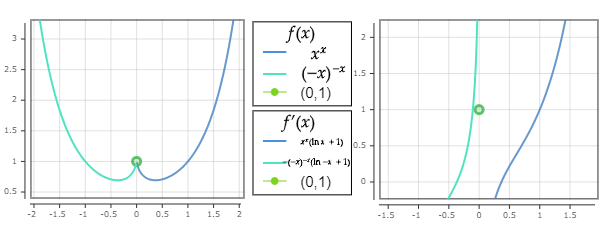
\includegraphics[scale=0.3]{build/pictures/dg3.png} 
}
\KRZ{Finde Taylorpolynom n-ter Ordnung}{ \begin{enumerate}
\item Definiere Entwicklungspunkt $a$ und zu approximierenden Punkt $x$.
\item Berechne $f'(x) , f''(x), \ldots ,f^{(n)}$
\item Setze ein:$f(a)+f'(a)(x-a)+ \frac{f''(a)(x-a)^2}{2}+\frac{f^{(3)}(a)(x-a)^3}{6}+\frac{f^{(4)}(a)(x-a)^4}{24} + \ldots + \frac{f^{(n)}(a)(x-a)^n}{n!}$
\end{enumerate}}
\KRZ{Finde Fehler des Taylorpolynoms}{ \begin{enumerate}
\item Definiere Entwicklungspunkt $a$ und zu approximierenden Punkt $x$.
\item Berechne $f^{(n+1)}$
\item Bilde Restpolynom $R = \frac{f^{(n+1)}(\xi)}{(n+1) !}(x-a)^{n+1}$
\item Finde $\xi \in ]a,x]$, so dass $R(\xi)$ maximal ist
\begin{itemize}
\item Suche lokales maximum ($f'(x)=0, f''(x)<0$)
\item Checke Ränder des Intervals
\end{itemize}

\end{enumerate}}




\mysection[magenta]{\centering Integralrechnung}
\DEF{5.1.1 (Partition)}{Eine Partition von $I$ ist eine endliche Teilmenge $P \subsetneq [a,b]$ wobei $\{a,b\} \subset P$.}
\DEF{ (Ober-/Untersumme)}{Wir definieren die Untersumme als
$$ s(f,P) := \sum_{i=1}^{n-1}f_i\delta_i \quad f_i = \inf_{x_{i-1}\leq x \leq x_i} f(x) $$
und die Obersumme:
$$ S(f,P) := \sum_{i=1}^{n-1}F_i\delta_i \quad F_i = \sup_{x_{i-1}\leq x \leq x_i} f(x) $$}
\LEM{5.1.2}{\begin{itemize}
\item[1.] Sei $P'$ eine Verfeinerung von $P$. Dann gilt: $s(f,P) \leq s(f,P') \leq S(f,P) \leq S(f,P')$ 
\item[2.] Für beliebige Partitionen $P_1$ und $P_2$ gilt $s(f,P_1) \leq S(f,P_2)$
\end{itemize}}
\DEF{5.1.3 (Integrierbarkeit)}{$f:[a,b] \longrightarrow \mathbb{R}$ für $a<b$ heisst Riemann integrierbar falls:
\begin{itemize}
\item[1.] $f$ ist auf $[a,b]$ beschränkt → $\exists M_1, M_2, \quad M_1 \leq f(x) \leq M_2$
\item[2.] $s(f) = S(f)$ , wir bezeichnen dann $s(f) = \int_a^b f(x)dx$\end{itemize} }
\SA{5.1.8 (Integrierbarkiet)}{$ f:[a,b] \longrightarrow \mathbb{R}$ ist integrierbar genau dann wenn $$\forall \varepsilon \exists \delta \quad \forall P \in P_{\delta} \left( [a,b]\right) \quad S(f,p) - s(f,p) < \epsilon  $$
wobei $P_{\delta} \left([a,b] \right)$ ist die Menge aller Partitionen mit Feinheit $\delta$}
\SA{5.2.1}{Seien $f, g:[a, b] \longrightarrow \mathbf{R}$ beschränkt, integrierbar und $\lambda \in \mathbf{R}$. Dann sind $f+g, \lambda \cdot f, f \cdot g,|f|, \max (f, g), \min (f, g)$ und $\frac{f}{g}($ falls $|g(x)| \geqslant \beta>0 \quad \forall x \in[a, b])$ integrierbar.}
\DEF{5.2.4 (gleichmässige Stetigkeit)}{DEFINITION 5.2.4. Eine Funktion $f: D \longrightarrow \mathbf{R}, D \subset \mathbf{R}$ ist in $D$ gleichmässig stetig, falls $\forall \varepsilon>0 \exists \delta>0 \quad \forall x, y \in D$ :
$$
|x-y|<\delta \Longrightarrow|f(x)-f(y)|<\varepsilon .
$$}
\SA{5.2.6 (Stetigkeit)}{Sei $f: [a,b] \longrightarrow \mathbf{R}$ stetig in dem kompakten Intervall $[a,b]$. Dann ist $f$ in $[a,b]$ gleichmässig stetig.}
\SA{5.2.7}{Sei $f:[a,b] \longrightarrow \mathbf{R}$ stetig. Dann ist $f$ integrierbar.}
\SA{5.2.8}{Sei $f:[a,b] \longrightarrow \mathbf{R}$ monoton. Dann ist $f$ integrierbar.}
\SA{5.2.10 (Linearität)}{Für $f,g:[a,b] \longrightarrow \mathbb{R}$, integrierbar $\alpha,\beta\in \mathbb{R}$
$\Rightarrow$ $\alpha f+ \beta g$ ist integrierbar und
$$ \int_{a}^{b} \left(\alpha f(x)+\beta g(x) dx \right) = \alpha\int_{a}^{b} f(x) dx + \beta \int_{a}^{b} g(x) dx  $$}
\SA{5.3.1}{Seien $f,g:[a,b] \longrightarrow \mathbb{R}$ beschränkt integrierbar, und $f(x) \leq g(x) \quad \forall x \in [a,b]$
Dann folgt:
$$ \int_{a}^{b} f(x)dx \leq \int_{a}^{b} g(x)dx $$}
\SA{5.3.2 (Dreiecksungleichung)}{Falls $f:[a,b] \longrightarrow \mathbb{R}$ beschränkt integrierbar, folgt
$$ \left| \int_{a}^{b} f(x)dx \right| \leq \int_{a}^{b} |f(x)|dx $$}
\SA{5.3.3 (Cauchy-Schwarz)}{Seien $f,g:[a,b] \longrightarrow \mathbb{R}$ beschränkt integrierbar. Dann gilt:
$$ \left| \int_{a}^{b}f(x)g(x)dx \right| \leq \sqrt{ \int_{a}^{b} f^2(x) } \sqrt{\int_{a}^{b} g^2(x)} $$}
\SA{5.4.1 }{Seien $a<b$ und $f:[a,b] \longrightarrow \mathbb{R}$ stetig. Die Funktionen
$$ F(x) = \int_{a}^{x} f(t) dt, \quad a\leq x \leq b $$
\begin{itemize}
\item $F(x)$ ist in $[a,b]$ stetig differenzierbar und
\item $F'(x) = f(x) \quad \forall x \in [a,b]$\end{itemize}}
\DEF{5.4.2 (Stammfunktion)}{Sei $a<b$ und $f:[a, b] \longrightarrow \mathbf{R}$ stetig. Eine Funktion $F:[a, b] \longrightarrow$ $\mathbf{R}$ heisst Stammfunktion von $f$, falls $F$ (stetig) differenzierbar in $[a, b]$ ist und $F^{\prime}=f$ in $[a, b]$ gilt.}
\SA{5.4.3 (Fundamentalsatz der Differentialrechnung)}{Sei $f:[a, b] \longrightarrow \mathbf{R}$ stetig. Dann gibt es eine Stammfunktion $F$ von $f$, die bis auf eine additive Konstante eindeutig bestimmt ist und es gilt:
$$
\int_a^b f(x) d x=F(b)-F(a)
$$}

\SA{5.4.5 (Partielle Integration)}{Seien $a<b$, $f,g:[a,b] \longrightarrow \mathbb{R}$ stetig differenzierbar. Dann gilt
$$ \int_{a}^{b} f'(x)g(x)dx = f(b)g(b)-f(a)g(a)-\int_{a}^{b} f(x)g'(x)dx  
$$}
\SA{5.4.6 (Integration durch Substitution)}{Sei $a<b$ , $g:[a,b] \longrightarrow \mathbb{R}$ stetig differerenzierbar, $I \in \mathbb{R}$ sodass $g \left([a,b] \right) \subset I$
Für $f:I \longrightarrow \mathbb{R}$ stetig gilt
$$ \int_{a}^{b}f(g(y))g'(y)dy = \int_{g(b)}^{g(a)} f(x)dx  $$}
\SA{5.5.1}{ Seien $a<b$, und $f_n:[a,b] \longrightarrow \mathbb{R}$ stetig für $n \geq 0$, $f:[a,b] \longrightarrow \mathbb{R}$.
Falls $f_n \longrightarrow f$ gleichmässig auf $[a,b]$ dann ist $f$ stetig und
$$ \int_{a}^{b} f(t)dt = \lim_{n \to \infty} \int_{a}^{b} f_n(x)  $$}
\COR{5.5.2}{Für eine Reihe $f(x) = \sum_{n=0}^\infty f_n(x)$ bedeutet dies:
$$ \int_{a}^{b} \left(\sum_{n=0}^{\infty}f_n(x) \right) dx = \sum_{n=0}^{\infty} \int_{a}^{b} f_n(x) dx $$ }
\COR{5.5.3}{Sei
$
f(x)=\sum_{n=0}^{\infty} c_k x^k
$
eine Potenzreihe mit positivem Konvergenzradius $\rho>0$. Dann ist für jedes $0 \leqslant r<\rho$, $f$ auf $[-r, r]$ integrierbar und es gilt $\forall x \in]-\rho, \rho[$ :
$$
\int_0^x f(t) d t=\sum_{n=0}^{\infty} \frac{c_n}{n+1} x^{n+1} .
$$}
\DEF{5.8.1 (Uneigentliche Integrale)}{ Für $f:[a,b[ \longrightarrow \mathbb{R}$ oder $f:]a,b] \longrightarrow \mathbb{R}$ ist integrierbar wenn
$$ \lim_{x \to b} \int_{a}^{x} f(t)dt \text{ oder } \lim_{x \to a} \int_{x}^{b} f(t)dt $$
existiert.
Man bezeichnet
$$ \int_{a}^{b} f(t)dt = \lim \int_{a}^{x} f $$
als uneigentliches Integral.}
\LEM{5.8.3}{Sei $f:[a, \infty[\longrightarrow \mathbf{R}$ beschränkt und integrierbar auf $[a, b] \quad \forall b>a$.
\begin{itemize}
\item[1.] Falls $|f(x)| \leqslant g(x) \quad \forall x \geqslant a$ und $g(x)$ ist auf $[a, \infty[$ integrierbar, so ist $f$ auf $[a, \infty[$ integrierbar.
\item[2.]  Falls $0 \leqslant g(x) \leqslant f(x)$ und $\int_a^{\infty} g(x) d x$ divergiert, so divergiert auch $\int_a^{\infty} f(x) d x$.
\end{itemize}}
\SA{5.8.5}{Sei $f:[1,\infty[ \longrightarrow [0,\infty[$ monoton fallend
Die Reihe $\sum_{n=1}^{\infty} f(n)$ ist konvergent $\Leftrightarrow$ $\int_{1}^{\infty} f(x) dx$ konvergiert}

\mysubsection{Kochrezepte Integral}

\DEF{(Akkumulationsfunktion)}{
Eine Akkumulationsfunktion ist eine Funktion in der Form:
$$ A(x) = \int_{c}^{x} f(z)dz
$$
Solange $f(z)dz$ stetig in $[c,x]$ ist gilt generell: $$A'(x)=f(x) $$
Kombiniert mit der Kettenregel folgt für eine allgemeinere Form der Funktion:
$$\frac{d}{dx} \int_{c}^{h(x)} f(z)dz = f(h(x))\cdot h'(x) = F(g(x))' $$
Ein Beispiel:
$$f(z)=\int_{0}^{x^2} \frac{1}{z^2+4}$$
hier ist $h(x)=x^2$. Somit folgt
$$\frac{d}{dx}\int_{0}^{x^2} \frac{1}{z^2+4} = \frac{1}{(x^2)^2+4}\cdot (x^2)' = \frac{2x}{x^4+4}$$
Wichtig ist anzumerken, dass die Funktion nur in der oberen Grenze eine Variabel haben kann. Falls man Funktionen in der Form $
 \int_{p(x)}^{h(x)} f(z)dz$
 antrifft kann man sie lösen indem man das Integral teilt:
 $$ \int_{p(x)}^{h(x)} f(z)dz = \int_{0}^{h(x)} f(z)dz - \int_{0}^{p(x)} f(z)dz  $$}
 
\KRZ{Unbestimmtes Integral mit Substitution}{
Man folge einfach den folgenden Schritten:
\begin{enumerate}
\item Bestimme $u := f(x)$
\item Berechne $du$ und löse für $dx$: $du = f'(x) \Rightarrow dx = \frac{du}{f'(x)}$
\item Substituiere $u$ und $du$ in die ursprüngliche Gleichung
\item Wenn sich nicht alle $x$ herauskürzen; löse für $x$ in der Gleichung des ersten Schrittes
\item Setze Schritt 4 ein.
\item Löse das Integral
\item Rücksubstituiere $x$
\end{enumerate}
Beispiel:\\
Gegeben sei $$\int x \sqrt{3x+2}dx$$
\begin{enumerate}
\item $u = 3x + 2$
\item $du = 3 \Rightarrow dx = \frac{du}{3}$
\item $\int x \sqrt{u} \frac{du}{3}$
\item $u = 3x + 2 \Rightarrow x = \frac{u-2}{3} $
\item $\int \frac{u-2}{3}\sqrt{u} \frac{du}{3}  $
\item
Die letzte Gleichung kann man relativ einfach lösen:
$$ \int \frac{u-2}{3}\sqrt{u} \frac{du}{3}   = \frac{1}{9} \int \left( u-2 \right) u^{\frac{1}{2}} du$$
$$ = \frac{1}{9} \int u^{\frac{3}{2}} - 2 u^{\frac{1}{2}} = \frac{1}{9} \left[\frac{2u^{\frac{5}{2}}}{5} - \frac{2 \cdot 2u^{\frac{3}{2}}}{3}\right]$$
$$ = \frac{2}{45}u^{\frac{5}{2}}-\frac{4}{27}u^{\frac{3}{2}}$$
\item 
$$  \frac{2}{45}u^{\frac{5}{2}}-\frac{4}{27}u^{\frac{3}{2}} = \frac{2}{45} \left[3x+2 \right]^{\frac{5}{2}}-\frac{4}{27}\left[3x+2 \right]^{\frac{3}{2}}$$
\end{enumerate}
}
\KRZ{Partielle Integration: DI-Methode}{
Gegeben sein die zu integrierenden Funktion $$\int f g$$
\begin{enumerate}
\item Wähle die zu integrierende Funktion $f$ und die zu differenzierende $g$ aus.
\item Fülle die Tabelle aus, bis:
\begin{enumerate}
\item man eine $0$ in der differenzierenden Spalte erhält
\item Eine Reihe integrierbar wird
\item Eine Reihe kommt ein zweites mal vor
\end{enumerate}
\begin{center}

\begin{tabular}{l|ll}
    & $D$ & $I$ \\ \hline
$+$   & $f$   & $g$   \\
$-$   &  $f'$ &  $\int g = g^{(-1)}$ \\ 
$+$   & $f''$  &   $g^{(-2)}$ \\ 
$\ldots$   &  &   \\ 
$\pm$ & $f^{(n)} = 0$  &  $g^{(-n)}$  \\ 
\end{tabular}
\end{center}
\item
\begin{enumerate}
\item Das Ergebnis lässt sich nun von der Tabelle ablesen, indem man die diagonalen produkte (von oben nach unten) aufsummiert. Es ergibt sich also:
$$f \cdot g^{(-1)} - f'\cdot g^{(-2)}  + \ldots  \pm f^{(n-1)}\cdot g^{(-n)}$$
\item Das Ergebnis lässt sich nun ebenfalls ablesen in dem man zuerst die diagonalen Produkte aufsummiert. Dies tut man so lange bis man zur Reihe kommt, in der das Produkt integriert werden kann. Man nehme an $f^{(n)} \cdot g^{(-n)}$ ist einfach integrierbar, dann ergibt sich:
$$ f \cdot g^{(-1)} - f'\cdot g^{(-2)}  + \ldots  \pm \int f^{(n)}\cdot g^{(-n)}$$
\item Das Ergebnis wird nun gleich berechnet wie bei (b), jedoch erhählt man eine Gleichung die man nach $\int fg$ auflösen kann.

\end{enumerate}

\end{enumerate}
}

\KRZ{Partialbruchzerlegung}{Seien $P, Q$ Polynome mit $grad(P) < grad(Q)$ und $Q$ mit der Produktzerlegung $Q(x) = \prod_{j = 1}^l \big( (x- \alpha_j)^2 + \beta_j^2\big)^{m_j} \prod_{i = 1}^k (x - \gamma_i)^{n_i}$. Dann gibt es $A_{ij}, B_{ij}, C_{ij}$ reelle Zahlen mit
$$
  \frac{P(x)}{Q(x)} = \sum_{i = 1}^l \sum_{j = 1}^{m_i} \frac{(A_{ij} + B_{ij}x)}{\big( (x- \alpha_i)^2 + \beta_i^2\big)^j} + \sum_{i = 1}^k \sum_{j = 1}^{n_i} \frac{C_{ij}}{(x-\gamma_i)^j}
$$
Bei einer Partialbruchzerlegung geht man folgendermassen vor:
\begin{enumerate}[(i)]
  \item Sei $R(x) = \frac{P(x)}{Q(x)}$. Falls $grad(P) \geq grad(Q)$ wenden wir Polynomdivision an.
  \item $Q$ lässt sich nun als $Q(x) = \prod_{j = 1}^l \big( (x- \alpha_j)^2 + \beta_j^2\big)^{m_j} \prod_{i = 1}^k (x - \gamma_i)^{n_i}$ zerlegen. Das sind
  die Komplexen und reelen Nullstellen mit ihrer vielfachheit.
  \item Wir bilden nun die "hässliche" Summe von oben
  \item Wir bestimmen mithilfe von Koeffizientenvergleich (Nennerpolynom Multiplizieren) die unbekannten $A_{ij}, B_{ij}, C_{ij}$.
\end{enumerate}
Hier ein einfaches Beispiel:
\begin{align*}
  &\frac{5x + 1}{x^2 + x - 2} = \frac{5x + 1}{(x - 1)(x + 2)} = \frac{A}{x - 1} + \frac{B}{x + 2}\\ \\
  &\Rightarrow \text{ Löse } 5x + 1 = A(x + 2) + B(x - 1)\\ \\
  &\Rightarrow \text{Setze } x = -2,\;1
\end{align*}
Mit mehreren Linearen Faktoren:
\begin{align*}
  &\frac{-2x^2 + x + 8}{x (x-2)^2} = \frac{A}{x} + \frac{B}{x - 2} + \frac{C}{(x-2)^2}\\ \\
  &\Rightarrow \text{ Löse } -2x^2 + x + 8 = A(x - 2)^2 + Bx(x - 2) + Cx
\end{align*}
Ohne reelle Nullstellen:
\begin{align*}
  &\frac{2x^2 -3x + 3}{(x-1)(x^2 + 1)} = \frac{A}{x - 1} + \frac{Bx + C}{x^2 + 1}\\ \\
  &\Rightarrow \text{ Löse } 2x^2 -3x + 3 = A(x^2 + 1) + (Bx + C)(x - 1)\\ \\
  &\Rightarrow \text{Setze } x = 0,\;1,\;2
\end{align*}}
\KRZ{Rationale Funktionen Integrieren}{
Wir betrachten einen Spezialfall der Partialbruchzerlegung.
Gegeben sei eine rationale Funktion $f(x)=\frac{P(x)}{Q(x)}$. Wir nehmen an das $deg(Q(x))=1$ und sich damit $Q(x)$ schreiben lässt als $(x - \alpha)$. Wir wollen $\int \frac{P(x)}{Q(x)}$ berechnen
\begin{enumerate}
\item Führe Polynomdivision $\frac{P(x)}{(x- \alpha)}$ aus. Wir nennen den Quotienten $q$ und den Rest $r$ wobei $deg(r)=0$
\item Schreibe um zu: $$\int\frac{P(x)}{Q(x)} = \int \frac{q (x-\alpha)}{(x-\alpha)}+ \int \frac{r}{(x-\alpha)}$$
\item Kürze und Integriere Separat: $$ \int \frac{q (x-\alpha)}{(x-\alpha)}+ \int \frac{r}{(x-\alpha)}= \int q  + r \int \frac{1}{(x-\alpha)}$$
 \item Es gelten generell: $$\int \frac{a}{x+b} dx = a \cdot \ln |x+b| $$ $$  \int (ax + b) dx = \frac{ax^2}{2	}+bx$$
\end{enumerate}
Hier ein Beispiel:

$$\int \frac{x^2-6x+8}{x+1}$$
\begin{enumerate}
\item $$(x^2-6x+8){x+1} = (x-7), r = -15$$
\item $$ \ldots = \int \frac{(x+1)(x-7)}{(x+1)} + \int \frac{-15}{(x-1)}$$
\item $$\ldots= \int (x-7) - \int \frac{1}{(x+1)}$$
\end{enumerate}
}


\section{Anhang}
\subsection{Trigonometrie}
\vspace{1mm} \hline \vspace{3 mm}
\subsubsection{Periodizität}
\begin{itemize}
 \item $\sin(\alpha + 2 \pi) = \sin(\alpha) \quad \cos(\alpha + 2 \pi) = \cos(\alpha)$
 \item $\tan(\alpha + \pi) = \tan(\alpha) \quad \cot(\alpha + \pi) = \cot(\alpha)$

\end{itemize}

\subsubsection{Parität}
\begin{itemize}
 \item $\sin(-\alpha) = - \sin(\alpha) \quad \cos(-\alpha) = \cos(\alpha)$
 \item $\tan(-\alpha) = - \tan(\alpha) \quad \cot(-\alpha) = - \cot(\alpha)$
\end{itemize}

\subsubsection{Ergänzung}
\begin{itemize}
 \item $\sin(\pi - \alpha) = \sin(\alpha) \quad \cos(\pi - \alpha) = - \cos(\alpha)$
 \item $\tan(\pi - \alpha) = -\tan(\alpha) \quad \cot(\pi - \alpha) = - \cot(\alpha)$
\end{itemize}


\subsubsection{Komplemente}
\begin{itemize}
 \item $\sin(\pi/2 - \alpha) = \cos(\alpha) \quad \cos(\pi/2 - \alpha) = \sin(\alpha)$
 \item $\tan(\pi/2 - \alpha) = -\tan(\alpha) \quad \cot(\pi/2 - \alpha) = -\cot(\alpha)$
\end{itemize}

\subsubsection{Doppelwinkel}
\begin{itemize}
 \item $\sin(2\alpha) = 2 \sin(\alpha) \cos(\alpha)$
 \item $\cos(2\alpha) = \cos^2(\alpha) - \sin^2(\alpha) = 1 - 2 \sin^2(\alpha)$
 \item $\tan(2\alpha) = \frac{2\tan(\alpha)}{1 - \tan^2(\alpha)}$
\end{itemize}

\subsubsection{Addition}
\begin{itemize}
 \item $\sin(\alpha + \beta) = \sin(\alpha) \cos(\beta) + \cos(\alpha) \sin(\beta)$
 \item $\cos(\alpha + \beta) = \cos(\alpha) \cos(\beta) - \sin(\alpha) \sin(\beta)$
 \item $\tan(\alpha + \beta) = \frac{\tan(\alpha) + \tan(\beta)}{1 - \tan(\alpha) \tan(\beta)}$
\end{itemize}

\subsubsection{Subtraktion}
\begin{itemize}
 \item $\sin(\alpha - \beta) = \sin(\alpha) \cos(\beta) - \cos(\alpha)\sin(\beta)$
 \item $\cos(\alpha - \beta) = \cos(\alpha) \cos(\beta) + \sin(\alpha)\sin(\beta)$
 \item $\tan(\alpha - \beta) = \frac{\tan(\alpha) - \tan(\beta)}{1+\tan(\alpha) \tan(\beta)}$
\end{itemize}

\subsubsection{Multiplikation}
\begin{itemize}
 \item $\sin(\alpha) \sin(\beta) = -\frac{\cos(\alpha + \beta) - \cos(\alpha - \beta)}{2}$
 \item $\cos(\alpha) \cos(\beta) =  \frac{\cos(\alpha + \beta) + \cos(\alpha - \beta)}{2}$
 \item $\sin(\alpha) \cos(\beta) =  \frac{\sin(\alpha + \beta) + \sin(\alpha - \beta)}{2}$
\end{itemize}

\subsubsection{Potenzen}
\begin{itemize}
 \item $\sin^2(\alpha) = \frac{1}{2}(1-\cos(2\alpha))$
 \item $\cos^2(\alpha) = \frac{1}{2}(1+\cos(2\alpha))$
 \item $\tan^2(\alpha) = \frac{1-\cos(2\alpha)}{1+\cos(2\alpha)}$
\end{itemize}

\subsubsection{Reduktion}
\begin{itemize}
\item $\sin^2(u) = \frac{1-\cos(2u)}{2}$
\item $\cos^2(u) = \frac{1+\cos(2u)}{2}$
\item $\tan^2(u) = \frac{1-\cos(2u)}{1+\cos(2u)}$

\item $\cos^3(u) = \frac{3 \sin(u)-\sin(3u)}{4}$
\item $\sin^3(u) = \frac{3 \sin(u)+\sin(3u)}{4}$
\item $\tan^3(u) = \frac{3 \sin(u)-\sin(3u)}{3 \sin(u)+\sin(3u)}$ 

\item $\cos^4(u) = \frac{3- 4 \cos(2u) + \cos(4u)}{8}$
\item $\sin^4(u) = \frac{3+ 4 \cos(2u) + \cos(4u)}{8}$
\item $\tan^4(u) = \frac{3- 4 \cos(2u) + \cos(4u)}{3+4 \cos(2u) + \cos(4u)}$
 
\item $\cos^5(u) = \frac{10 \sin(u) - 5 \sin(3u)+ \sin(5u)}{16}$
\item $\sin^5(u) = \frac{10 \sin(u) + 5 \sin(3u)+ \sin(5u)}{16}$
\item $\tan^5(u) = \frac{10 \sin(u) - 5 \sin(3u)+ \sin(5u)}{10 \sin(u) + 5 \sin(3u)+ \sin(5u)}$ 
\end{itemize}

\subsubsection{Diverse}

\begin{itemize}
 \item $\sin^2(\alpha) + \cos^2(\alpha) = 1$
 \item $\cosh^2(\alpha) - \sinh^2(\alpha) = 1$
 \item $\sin(z) = \frac{e^{iz} - e^{-iz}}{2i}$ und $\cos(z) = \frac{e^{iz} + e^{-iz}}{2}$
 \item $\exp (iz) = \cos(z) + i \sin(z)$
 \item $\tan(z)=\frac{\sin(z)}{\cos(z)}\quad \cot(z)=\frac{\cos(z)}{\sin(z)}$
 \item $sin(x)\leq x$
\end{itemize}
\begin{center} 
\subsubsection{Werte}
 \begin{tabular}{c|cccccc}
  deg& $0 \degree $ & $30 \degree $ & $45 \degree $ & $60 \degree $ & $90 \degree $ & $180 \degree $ \\
  \hline
  rad & 0 & $\frac{\pi}{6}$ & $\frac{\pi}{4}$ & $\frac{\pi}{3}$ & $\frac{\pi}{2}$ & $\pi$ \\
  cos & 1 & $\frac{\sqrt{3}}{2}$ & $\frac{\sqrt{2}}{2}$ & $\frac{1}{2}$ & 0 & -1 \\
  sin & 0 & $\frac{1}{2}$ & $\frac{\sqrt{2}}{2}$ & $\frac{\sqrt{3}}{2}$ & 1 & 0 \\
  tan & 0 & $\frac{1}{\sqrt{3}}$ & 1 & $\sqrt{3}$ & $+\infty$ & 0 \\
 \end{tabular}
\end{center} 
\subsubsection{Domain}
$$\sin: \left[\frac{-\pi}{2},\frac{\pi}{2} \right] \longrightarrow \left[-1,1\right]$$
 $$\cos: \left[0,\pi \right] \longrightarrow \left[-1,1\right]$$
$$\tan: \left[\frac{-\pi}{2},\frac{\pi}{2}\right] \longrightarrow \mathbb{R}$$
$$\sinh: \mathbb{R} \longrightarrow\mathbb{R} $$
 $$\cosh: \mathbb{R}\longrightarrow \left[1,\infty\right[$$
 $$\tanh: \mathbb{R}\longrightarrow \left[-1,1\right]$$

\subsubsection{Graph}



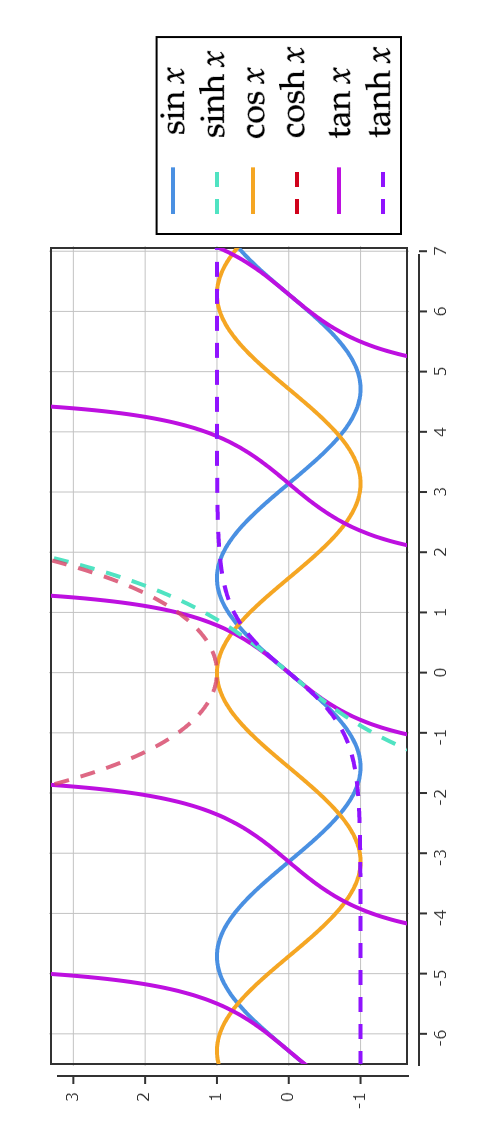
\includegraphics[scale=0.4]{build/pictures/dg1.png} 

\vspace{1mm} \hline \vspace{1 mm}



\subsection{Grenzwerte}
\begin{center}
  \begin{tabularx}{\linewidth}{XX}
    \toprule
    $\limxi \frac{1}{x} = 0$ & $\limxi 1 + \frac{1}{x} = 1$ \\
    $\limxi e^x = \infty$ & $\limxn e^x = 0$ \\
    $\limxi e^{-x} = 0$ & $\limxn e^{-x} = \infty$ \\
    $\limxi \frac{e^x}{x^m} = \infty$ & $\limxn xe^x = 0$ \\
    $\limxi \ln(x) = \infty$ & $\limxo \ln(x) = -\infty$ \\
    $\limxi (1+x)^{\frac{1}{x}} = 1$ & $\limxo (1+x)^{\frac{1}{x}} = e$ \\
    $\limxi (1+\frac{1}{x})^b = 1$ & $\limxi n^{\frac{1}{n}} = 1$ \\
    $\lim_{x\to\pm\infty} (1 + \frac{1}{x})^x = e$ & $\limxi (1-\frac{1}{x})^x = \frac{1}{e}$ \\
    $\lim_{x\to\pm\infty} (1 + \frac{k}{x})^{mx} = e^{km}$ & $\limxi (\frac{x}{x+k})^x = e^{-k}$ \\
    $\limxo \frac{a^x -1}{x} = \ln(a), \newline \forall a > 0$ &
    $\limxi x^a q^x = 0, \newline \forall 0 \le q < 1$ \\
    $\lim_{x \to \infty} \left(\frac{1+ na}{na} \right)^n = \sqrt[a]{e}$ & $\lim_{x \to \infty} \sqrt{ax^2 + bx+c}- \sqrt{a}x = \frac{b}{2 \sqrt{a}}$\\
  \end{tabularx}
  \begin{tabularx}{\linewidth}{XX}
    $\limxo \frac{\sin x}{x} = 1$ & $\limxo \frac{\sin kx}{x} = k$\\
    $\limxo \frac{1}{\cos x} = 1$ & $\limxo \frac{\cos x -1}{x} = 0$ \\
    $\limxo \frac{\log 1 - x}{x} = -1$ & $\limxo x \log x = 0$\\
    $\limxo \frac{1 - \cos x}{x^2} = \frac{1}{2}$ & $\limxo \frac{e^x-1}{x} = 1$ \\
    $\limxo \frac{x}{\arctan x} = 1$ & $\limxi \arctan x = \frac{\pi}{2}$ \\
    $\limxo \frac{e^{ax}-1}{x} = a$ & $\limxo \frac{\ln(x+1)}{x} = 1$ \\
    $\lim_{x\to 1} \frac{\ln(x)}{x-1} = 1$ & $\limxi \frac{\log(x)}{x^a} = 0$ \\
    $\limxi \sqrt[x]{x} = 1$ & $\limxi \frac{2x}{2^x} = 0$ \\
    \bottomrule
  \end{tabularx}
\end{center}

\subsection{Reihen}
\begin{center}
  \begin{tabularx}{\linewidth}{XX}
    \toprule
    $\sum_{i=1}^{n} i = \frac{n(n+1)}{2}$ & $\sum_{i=1}^{n} i^2 = \frac{n(n+1)(2n+1)}{6}$ \\
    $\sum_{i=1}^{n} i^3 = \frac{n^2 (n+1)^2}{4} $ & $\sum_{i=1}^{\infty} \frac{1}{i^2} = \frac{\pi ^2}{6}$ \\
    $\sum_{i=1}^{ \infty} \frac{1}{i (i+1	)} =1$ &$\sum_{i=0}^{\infty} x^i = \frac{1}{1-x}$\\
     $\sum_{n=0}^{\infty}\frac{(-1)^n}{2n+1} = \frac{\pi}{4}$& $\sum_{n=1}^{\infty}\frac{(-1)^{n+1}}{n} = \ln(2)$  \\
    
    
    \bottomrule
  \end{tabularx}
\end{center}




\subsection{Ableitungen}
\begin{center}
  % the c>{\centering\arraybackslash}X is a workaround to have a column fill up all space and still be centered
  \begin{tabularx}{\linewidth}{c>{\centering\arraybackslash}Xc}
  \toprule
  $\mathbf{F(x)}$ & $\mathbf{f(x)}$ & $\mathbf{f'(x)}$ \\
  \midrule
  $\frac{x^{-a+1}}{-a+1}$ & $\frac{1}{x^a}$ & $\frac{a}{x^{a+1}}$ \\
  $\frac{x^{a+1}}{a+1}$ & $x^a \ (a \ne -1)$ & $a \cdot x^{a-1}$ \\
  $\frac{1}{k \ln(a)}a^{kx}$ & $a^{kx}$ & $ka^{kx} \ln(a)$ \\
  $\ln |x|$ & $\frac{1}{x}$ & $-\frac{1}{x^2}$ \\
  $\frac{2}{3}x^{3/2}$ & $\sqrt{x}$ & $\frac{1}{2\sqrt{x}}$\\
  $\frac{n}{n+1}x^{\frac{1}{n}+1}$ & $\sqrt[n]{x}$ & $\frac{1}{n}x^{\frac{1}{n}-1}$\\
  $-\cos(x)$ & $\sin(x)$ & $\cos(x)$ \\
  $\sin(x)$ & $\cos(x)$ & $-\sin(x)$ \\
  $\frac{1}{2}(x-\frac{1}{2}\sin(2x))$ & $\sin^2(x)$ & $2 \sin(x)\cos(x)$ \\
  $\frac{1}{2}(x + \frac{1}{2}\sin(2x))$ & $\cos^2(x)$ & $-2\sin(x)\cos(x)$ \\
  \multirow{2}*{$-\ln|\cos(x)|$} & \multirow{2}*{$\tan(x) = \frac{\sin}{\cos}$} & $\frac{1}{\cos^2(x)}$  \\
  & & $1 + \tan^2(x)$ \\
  $\cosh(x)$ & $\sinh(x)$ & $\cosh(x)$ \\
  $\log(\cosh(x))$ & $\tanh(x)$ & $\frac{1}{\cosh^2(x)}$ \\
  $\ln | \sin(x)|$ & $\cot(x)$ & $-\frac{1}{\sin^2(x)}$ \\
  $\frac{1}{c} \cdot e^{cx}$ & $e^{cx}$ & $c \cdot e^{cx}$ \\
  $x(\ln |x| - 1)$ & $\ln |x|$ & $\frac{1}{x}$ \\
  $\frac{1}{2}(\ln(x))^2$ & $\frac{\ln(x)}{x}$ & $\frac{1 - \ln(x)}{x^2}$ \\
  $\frac{x}{\ln(a)} (\ln|x| -1)$ & $\log_a |x|$ & $\frac{1}{\ln(a)x}$ \\

  \bottomrule
  \end{tabularx}
\end{center}
\subsubsection{Besonders hässliche Ableitungen}
\begin{itemize}
 \item $\left(x^x\right)' = x^x \cdot(1+\ln x) \quad x>0$ 
\item $\left(\left(x^x\right)^x \right)'= \left(x^x\right)^x(x+2 x \ln (x)) \quad x>0$ 
\item $\left(x^{\left(x^x\right)} \right)'=x^{\left(x^x\right)}\left(x^{x-1}+\ln x \cdot x^x(1+\ln x)\right)$
\end{itemize}
\begin{center}
  \begin{tabularx}{\linewidth}{>{\centering\arraybackslash}X>{\centering\arraybackslash}X}
  \toprule
  $\mathbf{F(x)}$ & $\mathbf{f(x)}$ \\
  \midrule
  $\frac{1}{a\cdot (n+1)}(ax+b)^{n+1}$ & $(ax+b)^n$ \\
  
  $\arcsin(x)$ & $\frac{1}{\sqrt{1 - x^2}}$ \\
  $\arccos(x)$ & $\frac{-1}{\sqrt{1 - x^2}}$ \\
  $\arctan(x)$ & $\frac{1}{1 + x^2}$ \\ 
  $\text{arcsinh}(x)$ & $\frac{1}{\sqrt{1 + x^2}}$ \\
  $\text{arccosh}(x) $ & $\frac{1}{\sqrt{x^2 - 1}}$ \\
  $\text{arctanh}(x) $ & $\frac{1}{1 - x^2}$ \\ 
  $x^x \ (x > 0)$ & $x^x \cdot (1 + \ln x)$ \\
  $\log_a|x|$ & $\frac{1}{x \ln a}=\log_a(e)\frac{1}{x}$ \\
  \bottomrule
  \end{tabularx}
\end{center}

\subsection{Taylorpolynome }
\vspace{1mm} \hline \vspace{3 mm}
$T_n(f(x), x, x_0 )$ ist das Taylorpolynom $n$-ter Ordnung der Funktion $f(x)$ mit dem Entwicklungspunkt $x_0$ für das Argument $x$. Die Potenzreihenentwicklung ist ein analoger Begriff.
\begin{itemize}




\item  $T_{\infty}(\sin(x), x,0)= \sum_{n=0}^{\infty}(-1)^n \frac{x^{2n+1}}{(2n+1)!} = x - \frac{x^3}{6}+\frac{x^5}{120} \ldots$
\item
 $T_{\infty}(\cos(x), x,0)= \sum_{n=0}^{\infty}(-1)^n \frac{x^{2n}}{(2n)!} = 1- \frac{x^2}{2}+\frac{x^4}{24} \ldots $
 \item $T_{\infty}(e^{x}, x,0)= \sum_{n=0}^{\infty} \frac{(x)^n}{n!} = 1 + x + \frac{x^2}{2} \ldots $
  \item $T_{\infty}(e^{x+1}, x,0)= \sum_{n=0}^{\infty} \frac{(1+x)^n}{n!} = 1 + x + \frac{x^2}{2} \ldots $
 \item $T_{\infty}(\ln(x), x,1)=\sum_{n=1}^\infty \frac{(-1)^{n+1}}{n}(x-1)^n = (x-1) - \frac{(x-1)^2}{2} + \frac{(x-1)^3}{3} - \ldots$ für $0< x \leq 2$
 \item $T_{\infty}(\ln(1+x), x,0)=-\sum_{n=1}^{\infty}\frac{x^n}{n}=x- \frac{x^2}{2}+\frac{x^3}{3} - \ldots $
 \item $T_{\infty}(\sqrt[k]{x+1}, x,0)=-\sum_{n=0}^{\infty}\binom{k^{-1}}{n}x^n = 1 + \frac{x}{n}-\frac{(n-1)x^2}{2n^2} + \ldots $
 \item $T_{\infty}(\frac{ax^2}{(b-x)^3}, x,0)=\sum_{n=2}^{\infty}\frac{a(n-1) \cdot n  \cdot x^n}{2b^{n+1}}   = \frac{ax^2}{b^3}+\frac{3ax^3}{b^4}+\frac{6ax^4}{b^5} + \ldots $
 \item $T_{\infty}(\frac{ax}{(b-x)^2}, x,0)=\sum_{n=1}^{\infty}\frac{n \cdot x^n }{b^{n+1}} = \frac{ax}{b^2}+\frac{2ax^2}{b^3}+\frac{3ax^3}{b^4} + \ldots $
\end{itemize}
  

\vspace{1mm} \hline \vspace{1mm}

\subsection{Integrale}
\begin{center}
 \begin{tabularx}{\linewidth}{>{\centering\arraybackslash}X>{\centering\arraybackslash}X}
  \toprule
  $\mathbf{f(x)}$ & $\mathbf{F(x)}$ \\
  \midrule
  $\int f'(x) f(x) \dx$ & $\frac{1}{2}(f(x))^2$ \\
  $\int \frac{f'(x)}{f(x)} \dx$ & $\ln|f(x)|$ \\
  $\int_{-\infty}^\infty e^{-x^2} \dx$ & $\sqrt{\pi}$ \\
  $\int (ax+b)^n \dx$ & $\frac{1}{a(n+1)}(ax+b)^{n+1}$ \\
  $\int x(ax+b)^n \dx$ & $\frac{(ax+b)^{n+2}}{(n+2)a^2} - \frac{b(ax+b)^{n+1}}{(n+1)a^2}$ \\
  $\int (ax^p+b)^n x^{p-1} \dx$ & $\frac{(ax^p+b)^{n+1}}{ap(n+1)}$ \\
  $\int (ax^p + b)^{-1} x^{p-1} \dx$ & $\frac{1}{ap} \ln |ax^p + b|$ \\
  $\int \frac{ax+b}{cx+d} \dx$ & $\frac{ax}{c} - \frac{ad-bc}{c^2} \ln |cx +d|$ \\
  $\int \frac{1}{x^2+a^2} \dx$ & $\frac{1}{a} \arctan \frac{x}{a}$ \\
  $\int \frac{1}{x^2 - a^2} \dx$ & $\frac{1}{2a} \ln\left| \frac{x-a}{x+a} \right|$ \\
  $\int \sqrt{a^2+x^2} \dx $ & $\frac{x}{2}f(x) + \frac{a^2}{2}\ln(x+f(x))$ \\

   
%here   
   
   
  $\int \frac{1}{(x+a)^2}dx$& $-\frac{1}{a+x}$ \\
$\int \frac{1}{(x+a)^3}dx$& $-\frac{1}{2(a+x)^2}$ \\
$\int \frac{1}{(x+a)^t}dx$& $\frac{1}{(1-t)(x+a)^{t+1}}$ \\
$\int \frac{x}{(x+a)^2}dx$& $\frac{a}{a+x}+\log |a+x|$ \\
$\int \frac{x}{(x+a)^3}dx$& $-\frac{a+2x}{2(a+x)^2}$ \\
$\int \frac{1}{ax^2+bx+c}dx$& $\frac{2 \arctan\left(\frac{2ax+b}{\sqrt{4ac-b^2}} \right)}{\sqrt{4ac-b^2}}$\\

  $\int \sin(kx)\cdot \cos(kx)dx$ & $-\frac{1}{4k}\cos(2kx)=\frac{-(\cos(x))^2}{2}$\\
  


 $\int \cos^n(x) d x$ & $\frac{n-1}{n} \int \cos^{n-2}(x) d x+\frac{\cos^{n-1}(x) \sin (x)}{n}$ \\
$ \int \sin^n(x) d x $ & $\frac{n-1}{n} \int \sin ^{n-2}(x) d x-\frac{\cos (x) \sin ^{n-1}(x)}{n}$\\


$\int \sin \cos dx$ & $\frac{-1}{2}\cos^2$\\
  $\int \frac{\cos}{ \sin} dx$ & $\log(\cos(x))$\\
  
  \bottomrule
 \end{tabularx}
\end{center}
\begin{flushleft}
\subsection{\colorbox{yellow!30}{Wichtig}}
\begin{itemize}
\item bei Grenzwerten immer beide Limit testen ($\lim_{x \to 0^{+}}$ und $\lim_{x \to 0^{-}} $)
\end{itemize}
\tiny
\subsection{Beispiele}
\vspace{1mm} \hline \vspace{3mm}
\subparagraph{Konvergenz von Reihen}
Seien $\sum_{k=1}^{\infty} a_k$ und $\sum_{k=1}^{\infty} b_k$ Reihen so dass $\sum_{k=1}^{\infty} a_k$ absolut konvergiert; $\sum_{k=1}^{\infty} b_k$ konvergiert.
Folgt daraus, dass
$$
\sum_{k=1}^{\infty} b_k \sin \left(a_k\right)
$$
konvergiert? Falls ja, muss die Aussage bewiesen werden. Falls nein, muss ein begründetes Beispiel gegeben werden.
\\
Zuerst beweisen wir dass $\lim_{k\to \infty}b_k = 0$:
Dazu konstruieren wir $c_k$ mit $c_1=0$ und $c_k = k_{k-1} \forall k\geq 2$. Da $\sum_{k=1}^{\infty} b_k$ konvergiert muss auch $\sum_{k=1}^{\infty} c_k$ konvergieren. Somit folgt:
$\lim_{n \to \infty}\sum_{k=1}^{0} b_k = \lim_{n \to \infty}\sum_{k=1}^{0} c_k $ und weiter gilt $\lim_{n \to \infty} b_n = \lim_{n \to \infty} \left(\sum_{k=1}^{0} b_k - \sum_{k=1}^{0} c_k  \right)=0$.\\
Da gilt $|\sin(x)| \leq |x|$ und $\sum_{k=1}^{\infty} a_k$ absolut konvergiert muss auch $\sum_{k=1}^{\infty}  \sin(a_k)$ konvergieren. Da $b_k$ konvergiert ist sie begrenzt durch eine Konstante $C$, gemäss S.2.2.2 (Weierstrass). Somit gilt $b_n \sin(a_n) \leq C |a_n|$. Da $a_n$ absolut konvergiert und die Ungleichheit gilt, konvergiert die gegebene Reihe ebenfalls.
\vspace{1mm} \hline \vspace{1mm}
\subparagraph{Konvergenz von Folgen}
Es sei $(a_n)_{n\geq 1}$ eine Folge positiver reeler Zahlen, sodass $\sum_{n=1}^{\infty} a_n$ konvergiert.
\begin{itemize}
\item[(i)] Geben Sie ein Beispiel einer Folge $a_n$ wie oben, welches zeigt, dass $\sum_{0}^{\infty} \sqrt{a_n}$ nicht konvergieren muss.
\item[(ii)] Zeigen Sie, dass für alle $n \geq 1$ gilt $\frac{\sqrt{a_n}}{n} \leq \operatorname{max}\{a_n, n^{-2}\}$
\item[(iii)] Beweisen Sie, dass $\sum_{n=1}^{\infty} \frac{\sqrt{a_n}}{n}$ absolut konvergiert.
\end{itemize}
\begin{itemize}
\item[(i)] Man betrachte die Folge $\sum_{n=1}^{\infty} \frac{1}{n^2}$ welche konvergiert zu $\frac{\pi^2}{6}$ jedoch ist $\sum_{n=1}^{\infty} \sqrt{\frac{1}{n^2}} =\sum_{n=1}^{\infty}  \frac{1}{n}  $ nicht konvergent.
\item[(ii)] Beweis durch Fallunterscheidung: \\ Fall 1: $a_n < \frac{\sqrt{a_n}}{n}$\\ Dann folgt  $a_n^2 < \frac{a_n}{n^2} \Rightarrow a_n < \frac{1}{n^2}$ im zweiten Fall gilt dann trivialerweise dass $a_n \geq \frac{\sqrt{a_n}}{n}$. Und somit gilt ebenfalls das zu beweisende Statement
\item[(iii)] Da $\sum_{n=1}^{\infty} a_n$ und $\sum_{n=1}^{\infty} n^{-2}$ absolut konvergente Reihen sind kann man die Summationsreihenfolge verändern und somit gilt:
\begin{align*}
\sum_{n=1}^{\infty} \frac{\sqrt{a_n}}{n} &\leq \sum_{n=1}^{\infty} \operatorname{max}\{a_n, n^{-2}\} \\ &\leq \sum_{n=1}^{\infty} a_n + n^{-2} \\ &=  \sum_{n=1}^{\infty} a_n + \sum_{n=1}^{\infty} n^{-2} 
\end{align*} Gemäss dem Vergleichssatz folgt somit die Behauptung
\end{itemize}
\vspace{1mm} \hline \vspace{1mm}
\subparagraph{Integration durch Substitution}
Beispiel 1:\\
Berechne $$\int_{e}^{e^e} \frac{\ln(\ln(x))}{x \ln(x)}$$
Integration durch Substitution, wobei gilt
\begin{itemize}
\item $f(x)=x$
\item $g(x) = \ln(\ln(x))$
\item $g'(x) =  \frac{1}{x \ln(x)}$
\end{itemize}
und somit gilt
$$\int_{g(0)}^{g(1)} f(y)dy = \int_{0}^{1} x dx = \frac{1}{2}$$ 
Beispiel 2:\\
Gegeben sei $$\int \frac{e^x}{e^{2x}+2e^x+1}$$
Wir formen um zu
$\int \frac{e^x}{e^{2x}+2e^x+1} = \frac{e^x}{(e^x+1)^2}$ und somit haben wir $u = (e^x+1)$ und $du=e^x$. Wir integrieren
$$\int \frac{e^x}{e^{2x}+2e^x+1}=\int \frac{1}{u^2}du = -\frac{1}{u} = -\frac{1}{e^x+1}$$
Beispiel 3:\\
$$\int \frac{1}{\sqrt{x}(1+x)}$$. Wir substituieren $u = \sqrt{x}$ und $du = \frac{1}{2\sqrt{x}} dx$ und somit ist $c=\frac{1}{2} \Rightarrow c^{-1} = 2$. Es folgt $$\int \frac{1}{1+u^2} du = 2\arctan(u) = 2\arctan(\sqrt{x})$$
Beispiel 4:\\
$$\int_{0}^{1} x \arcsin(x) dx$$
Wir substituieren:
\begin{itemize}
\item $u \arcsin(x), x = \sin(u)$
\item $dx = \cos(u)du$
\end{itemize}
und erhalten:
$$\int_{\arcsin(0)}^{\arcsin(1)} \sin(u) \arcsin(\sin(u)) \cos(u) = \int_{0}^{\frac{\pi}{2}} \sin(u) \cdot u \cdot \cos(u) du$$
Wir versuchen nun mit partielle Integration zwei Funktionen zu finden, die das Integral vereinfachen. Wir bemerken, dass die Funktion $u$ abgeleitet $1$ ergibt und wir somit nur noch $\sin \cos$ "integrieren müssen". Denn wenn $g(u)=u$ und somit $g'(u)=1$ gilt ergibt das:
$$\int u \sin(u) \cos(u) = fg - \int 1 \cdot f $$
Da gilt $ g =u$ bleibt noch $f=\sin \cos$. Somit ergibt sich:
$$ \int_{0}^{\frac{\pi}{2}} \underbrace{u}_{g} \underbrace{\sin(u) \cos(u)}_{f'} = \left. fg \right|_{0}^{\frac{\pi}{2}} -  \int_{0}^{\frac{\pi}{2}} \underbrace{1}_{g'} \cdot \underbrace{\frac{\sin^2(u)}{2}}_{f}  $$
Numerisch ergibt das folglich $\frac{\pi}{4}-\frac{\pi}{8}=\frac{\pi }{4}$
\vspace{1mm} \hline \vspace{1mm}
\subparagraph{Partielle Integration: DI-Methode}

Fall (a):\\
$$I = \int x^2 \sin(3x)dx$$
\begin{enumerate}
\item integrierende: $f=\sin(3x)$ und differenzierende: $g=x^2$
\item 
\begin{center}

\begin{tabular}{l|ll}
    & $D$ & $I$ \\ \hline
$+$   & $x^2$   & $\sin(3x)$   \\
$-$   &  $2x$ &  $\frac{-1}{3}\cos(3x)$ \\ 
$+$   & $2$  &   $\frac{-1}{9} \sin(3x)$ \\ 
$-$   & $0$ &  $\frac{1}{27}  \cos(3x)$ \\ 

\end{tabular}
\end{center}
\item 
$$I = \frac{-x^2}{3}\cos(3x)+ \frac{2x}{9}\sin(3x)+\frac{2}{27}\cos(3x)+C$$
\end{enumerate}
Fall (b):\\
$$I = \int x^4 \ln(x)dx$$
\begin{enumerate}
\item integrierende: $f=\ln(x)$ und differenzierende: $g=x^4$
\item
\begin{center}
\begin{tabular}{l|ll}
    & $D$ & $I$ \\ \hline
$+$   & $\ln(x)$   & $x^4$   \\
$-$   &  $\frac{1}{x}x$ &  $\frac{1}{5}x^5$ \\ 
 \end{tabular}
\end{center}
\item
$$I= \ln(x)\cdot \frac{1}{5}x^5 - \int \frac{1}{x} \frac{1}{5}x^5 dx = \ldots = \frac{\ln(x) x^5}{5} - \frac{1}{25}x^5 +C$$

\end{enumerate}
Fall (c):\\
$$I= \int e^x \sin(x) $$
\begin{enumerate}
\item integrierende: $f=\sin(x)$ und differenzierende: $g=e^x$
\item 
\begin{center}

\begin{tabular}{l|ll}
    & $D$ & $I$ \\ \hline
$+$   & $e^x$   & $\sin(x)$   \\
$-$   &  $e^x$ &  $-\cos(x)$ \\ 
$+$   & $e^x$  &   $- \sin(x)$ \\ 

\end{tabular}
\end{center}
\item \begin{align*}
I &= -e^{x} \cos(x) + e^x \sin(x) - I \\  2 I &= -e^{x} \cos(x) + e^x \sin(x)\\
I &= \frac{1}{2} \left[ -e^{x} \cos(x) + e^x \sin(x)\right]
\end{align*}
\end{enumerate}

\vspace{1mm} \hline \vspace{1mm}
\subparagraph{Limits }\\
Zeigen Sie, dass für alle $t \in \mathbb{R}$ gilt
$$
\lim _{n \rightarrow \infty}\left(\cos \left(\frac{t}{\sqrt{n}}\right)\right)^n=e^{-\frac{t^2}{2}} .
$$
Da $\cos (x)=1-\frac{x^2}{2}+\mathcal{O}\left(x^4\right)$ und $\log (1+x)=x+\mathcal{O}\left(x^2\right)$ gilt für alle $t \in \mathbb{R}$ wenn $n \rightarrow \infty$
$$
\begin{aligned}
\cos \left(\frac{t}{\sqrt{n}}\right)^n & =\exp \left(n \log \left(\cos \left(\frac{t}{\sqrt{n}}\right)\right)\right) \\
& =\exp \left(n \log \left(1-\frac{t^2}{2 n}+\mathcal{O}\left(\frac{1}{n^2}\right)\right)\right) \\
& =\exp \left(n\left(-\frac{t^2}{2 n}+\mathcal{O}\left(\frac{1}{n^2}\right)\right)\right) \\
& =\exp \left(-\frac{t^2}{2 n}+\mathcal{O}\left(\frac{1}{n^2}\right)\right) \underset{n \rightarrow \infty}{\longrightarrow} \exp \left(-\frac{t^2}{2}\right)=e^{-\frac{t^2}{2}}
\end{aligned}
$$

\subsection{Multiple Choice}
\vspace{1mm} \hline \vspace{3mm}
Für eine Folge $(a_n)$ mit $a_n \in \mathbb{R}$ für alle $n \in \mathbb{N}$, ist die Aussage $\lim_{n \to \infty } a_n = \infty$ äquivalent zu:
\begin{itemize}
\item[\textcolor{green}{C}]$\forall K \in \mathbb{N} \exists N \in \mathbb{N}$, so dass $\forall n \geq N: a_n \leq-K$
\item[\textcolor{red}{W}]$\forall \epsilon>0 \exists N \in \mathbb{N}$, so dass $\forall n \geq N:\left|a_n\right|<\epsilon$.
\item[\textcolor{red}{W}]$\forall N \in \mathbb{N} \exists K \in \mathbb{N}$, so dass $\forall n \geq N: a_n \leq-K$.
\item[\textcolor{red}{W}]$\forall N \in \mathbb{N} \exists \epsilon>0$, so dass $\forall n \geq N:\left|a_n\right|<\epsilon$.
\end{itemize} 
\vspace{1mm} \hline \vspace{1mm}
Welche der folgenden Reihen konvergieren?
\begin{itemize}
\item[\textcolor{red}{W}]$ \sum_{n=1}^{\infty} \frac{2018}{n} $ \textcolor{Emerald}{ $= 2018\cdot \sum_{n=1}^{\infty} \frac{1}{n}$ und die harmonische Reihe divergiert}
\item[\textcolor{green}{C}]$ \sum_{n=1}^{\infty} \frac{2018^n}{n !} $\textcolor{Emerald}{$= \exp(2018)$}
\item[\textcolor{red}{W}]$\sum_{n=1}^{\infty} \frac{e^n}{n^{2018}} $\textcolor{Emerald}{ divergiert da $\lim_{n \to \infty} \frac{e^n}{2018^n} = \infty$}
\item[\textcolor{green}{C}] $\sum_{n=1}^{\infty} \frac{\cos ((2018 n) !)}{n^2+1}$\textcolor{Emerald}{ $\leq  \sum_{n=1}^{\infty} \frac{1}{n^2}$ und dies konvergiert zu $\frac{\pi^2}{6}$}
\end{itemize}

\vspace{1mm} \hline \vspace{1mm}
Sei $f:[0,1] \to [0,1]$ stetig und nicht konstant. Dann gilt:
\begin{itemize}
\item[\textcolor{green}{C}] Es gibt einen Punkt $x \in [0,1]$, so dass $f(x)=x$.\textcolor{Emerald}{$g(x)= f(x)-x$. Da gilt $f(0),f(1) \in [0,1]$ folgt $g(0)=f(0)-0 \geq 0-0  = 0$ und $g(1) = f(1)-1 \leq 1-1 = 0$. Somit folgt aus dem Zwischenwertsatz (S.3.3.1) die Behauptung.}
\item[\textcolor{red}{W}]Es gibt einen Punkt $x \in [0,1]$, so dass $f(x)=1$.
\textcolor{Emerald}{Gegenbeispiel: $f(x)= \frac{x}{2}$}
\item[\textcolor{red}{W}] $f$ hat eine eindeutige Maximalstelle.
\textcolor{Emerald}{Gegenbeispiel: $f(x) = \frac{\sin(4\pi x)+1}{2}$}
\item[\textcolor{green}{C}] Das Bild $f([0,1]) \subset [0,1]$ ist ein abgeschlossenes Intervall. D.h es gibt $a,b \in [0,1]$ mit $a < b$, so dass $f([0,1]) = [a,b]$.
\textcolor{Emerald}{Gemäss dem Min-Max-Satz (S.3.4.5) hat $f$ auf $[0,1]$ ein Maximum $M$ und Minimum $m$. Gemäss dem Zwischenwertssatz (S.3.3.1) folgt $f([a,b]) = [m,M]$ und die Behauptung. }
\end{itemize}

\vspace{1mm} \hline \vspace{1mm}
Sei $f: \mathbb{R} \to \mathb{R}$ stetig. Dann gilt:
\begin{itemize}


\item[\textcolor{red}{W}] $f$ hat eine Maximalstelle.\textcolor{Emerald}{ Gegenbeispiel: $f(x)=x$}
\item[\textcolor{green}{C}] Wenn $f(1) = 2$ und $f(3) = -1$, dann gibt es ein $t\in]1,3[$ mit $f(t) = 0$.\textcolor{Emerald}{Folgt aus dem Zwischenwertssatz (S.3.3.1).}
\item[\textcolor{green}{C}] Wenn $\lim_{t \to \infty} f(t) = 0$ gilt, dann ist $f$ auf $[0,\infty[$ begrenzt.

\item[\textcolor{red}{W}] Wenn $f$ begrenzt ist, dann existiert $\lim{t \to \infty} f(t)$ \textcolor{Emerald}{Gegenbeispiel: $f(x) = \sin(x)$}
\end{itemize}
\vspace{1mm} \hline \vspace{1mm}
Seien $\left(a_n\right)_{n \in \mathbb{N}}$ und $\left(b_n\right)_{n \in \mathbb{N}}$ zwei Folgen mit $a_n, b_n \in \mathbb{R}$ für alle $n \in \mathbb{N}$. Welche der folgenden Antwortmöglichkeiten sind korrekt?
\begin{itemize}



\item[\textcolor{red}{W}]Wenn $a_n \leq b_n$ für alle $n \in \mathbb{N}$ und $\left(a_n\right)_{n \in \mathbb{N}}$ konvergent ist, dann ist auch $\left(b_n\right)_{n \in \mathbb{N}}$ konvergent. \textcolor{Emerald}{Gegenbeispiel: $a_n = n$ und $b_n=n$}

\item[\textcolor{green}{C}]Wenn $0 \leq b_n \leq a_n^3$ für alle $n \in \mathbb{N}$ und $a_n \rightarrow 0$ für $n \rightarrow \infty$, dann konvergiert auch $\left(b_n\right)_{n \in \mathbb{N}}$.\textcolor{Emerald}{Aus der Konvergenz von $a_n$ folgt $\lim_{n \to \infty} a_n^3 = 0 $. Mit dem Squeeze-Theorem folgt aus $0 \leq b_n \leq a_n^3$, dass $\lim_{n \to \infty} b_n = 0$}

\item[\textcolor{red}{W}]Wenn $\left|a_n-b_n\right| \leq \frac{1}{n}$ für alle $n \in \mathbb{N}$, dann konvergieren beide Folgen $\left(a_n\right)_{n \in \mathbb{N}}$ und $\left(b_n\right)_{n \in \mathbb{N}}$. \textcolor{Emerald}{Gegenbeispiel: $a_n=b_n=n$} 

\item[\textcolor{red}{W}]Wenn $\left(b_n^2\right)_{n \in \mathbb{N}}$ konvergiert, dann konvergiert auch $\left(b_n\right)_{n \in \mathbb{N}}$. \textcolor{Emerald}{Gegenbeispiel: $a_n=(-1)^n, a_n$ divergiert jedoch konvergiert $a_n^2 = 1$ } 
\end{itemize}
\vspace{1mm} \hline \vspace{1mm}



Sei $f:[0, \infty[\rightarrow \mathbb{R}$ stetig. Dann gilt:
\begin{itemize}

\item[\textcolor{green}{C}] Es gibt eine differenzierbare Funktion $F:] 0, \infty\left[\rightarrow \mathbb{R}\right.$ mit $F^{\prime}(t)=f(t)$ für alle $t \in] 0, \infty[$. \textcolor{Emerald}{Da $f$ stetig ist, ist $F(t) = \int_{0}^{t} f(s)ds$ wohledfiniert. Aus dem Fundamentalsatz der Algebra  folgt $  \forall t \in \mathbb{R}  \quad F'(t) = f(t) $}

\item[\textcolor{green}{C}] Wenn $f(t) \geq 0$ für alle $t \in[0,1]$ und $\int_0^1 f(t) d t=0$, dann gilt $f(t)=0$ für alle $t \in[0,1]$.
\textcolor{Emerald}{Wir definieren $F(t) = \int_{0}^{t}f(s)ds$. Da $f$ stetig ist, gilt $\forall t \in \mathbb{R} \quad F'(t)=f(t)$}. Zusätzlich ist $f$ wachsend da $f(t) \geq 0$. Es gilt $F(1) = F(0) = 0$ somit folgt $\forall t \in \mathbb{R} \quad F(t) = 0 $ und schliesslich $F'(t)=0$
\item[\textcolor{red}{W}] Wenn $|f(t)| \leq \frac{1}{t+1}$ für alle $t \in\left[0, \infty\left[\right.\right.$, dann existiert $\int_0^{\infty} f(t) d t$.
\textcolor{Emerald}{Gegenbeispiel: $f(t) = \frac{1}{t+1}$ mit $\int_{0}^{\infty} f(t) = \infty$ jedoch gilt trivialerweise die Bedingung}
\item[\textcolor{red}{W}] Wenn $\sum_{n=1}^{\infty} f(n)$ konvergiert, dann existiert $\int_0^{\infty} f(t) d t$.
\textcolor{Emerald}{Gegenbeispiel: $f(t) = \sin^2(\pi t) \Rightarrow \sum_{n=0}^{\infty}f(n) = 0$ jedoch $\int_{0}^{\infty} f(t) = \infty$}

\end{itemize}








\end{flushleft}

   \end{multicols}

\item[\textcolor{red}{W}]
\item[\textcolor{green}{C}]









\end{document}